\chapter{Results}
\lettrine[lines=1]{O}{ver}
 a span of 51 years, from 1973 to 2024, prominent themes have emerged and endured. Notably, biology, chemistry, environmental science, and materials science have consistently dominated the landscape, showcasing their enduring significance. 
%TC:ignore
\begin{table}[H]

    \caption{Science Takes Center Stage (1973-2024)}
    \label{tab: Topic List}

    \begin{adjustbox}{width=\textwidth} 
        \begin{tabular}{ *{5}{c} } 

            \midrule
            Material Science	&	Physics	&	Business	&	Developmental Biology	&	Political Science	\\
Medicine	&	Imaging Techniques	&	Automotive	&	Climate Science	&	Sensor Technology	\\
Epidemiology	&	Media Studies	&	Environmental Science	&	Development	&	Chemistry	\\
Philosophy	&	Infrastructure	&	Neuroscience	&	Ecology	&	Climate Science	\\
Microbiology	&	Particle Physics	&	Evolutionary Biology	&	Optics	&	Quantum Physics	\\
Biochemistry	&	Statistics	&	Computer Science	&	Manufacturing	&	Agriculture	\\
Healthcare	&	Machine Learning	&	Public Health	&	Networking	&	Astronomy	\\
Material Science	&	Biochemistry	&	Pediatrics	&	Immunology	&	Food Science	\\
Education	&	Oncology	&	Waste Management	&	Electronics	&	Oceanography	\\
Molecular Biology	&	Modeling	&	Mathematics	&	Geology	&	Surgery	\\

            \bottomrule
        \end{tabular}
    \end{adjustbox}
\end{table}
%TC:endignore
While this analysis provides valuable insights, it's important to acknowledge that the vast temporal scope might limit the depth of information attained. \\

I partitioned the metadata into consecutive three-year periods to gain deeper insights into the evolving landscape for a more concentrated exploration of the dominant trends and subjects influencing research and innovation within these specific timeframes. This focused examination of shorter intervals will provide a finer-grained and more intricate viewpoint. 

I have made six significant findings by analyzing and consolidating each triennial topic. 

\begin{enumerate}

  \item Sustained Importance: The topics of Environmental Science, Computer Science, Data Science, Ecology, Biology, and Training are consistently present throughout various periods, emphasizing their enduring significance and impact.

  \item Transient Topics: Some projects have emerged briefly during specific years, such as video games and supply chain disruptions in 2019-2021.

  \item Environment and Sustainable Development: During 2016-2018, there was a pinnacle of concern regarding environmental issues. The prevailing topics of that era were predominantly associated with the environment, including environmental science, earth science, ecology, energy materials, waste management, energy transfer, earth and geology, etc.

  \item Data science, computer science, and machine learning have repeatedly emerged at various time intervals.

  \item Limited Presence of Social Sciences: Public policy is a prominent funded focus within social science.

  \item Certain topics experienced fluctuations in attention across different years. For instance, Particle Physics was prominent in earlier years but waned later.\\
  
\end{enumerate}
%TC:ignore
\begin{table}[H]

    \caption{Topic List}
    \label{tab: Topic List}

    \begin{adjustbox}{width=\textwidth} 
        \begin{tabular}{ *{5}{c} } 
            \toprule
            2010-2012 & 2013-2015 & 2016-2018 & 2019-2021 & 2022-2024 \\
            \midrule
            Imaging	&	Machine Learning	&	Human-Computer Interaction	&	Problem Solving	&	Environmental Engineering	\\
Diagnostic Technology	&	Medical Technology	&	Healthcare	&	Agriculture	&	Medical Science	\\
Computer Science	&	Automotive Engineering	&	Transportation	&	Genetics	&	Engineering	\\
Neuroscience	&	Environmental Science	&	Environmental Science	&	Particle Physics	&	Microbiology	\\
Electronics	&	Neuroscience	&	Neuroscience	&	Natural Hazards	&	Mathematics	\\
Materials Science	&	Climate Science	&	Earth Science	&	Climate Resilience	&	Sports Science	\\
Environmental Science	&	Environmental Monitoring	&	Sensors and Monitoring	&	Data sensing	&	Physics	\\
Atmospheric Science	&	Ecology	&	Ecology	&	Quantum Technology	&	Agriculture	\\
Oceanography	&	Cell Biology	&	Cell Biology	&	Astrophysics	&	Plant Science	\\
Analytical Chemistry	&	Fluid Dynamics	&	Particle Chemistry	&	Protein Structure	&	Molecular Biology	\\
Bioinformatics	&	Cybersecurity	&	Network Security	&	Medical Diagnostics	&	Health Science	\\
Pharmaceutical Science	&	Plant Science	&	Agriculture	&	Soil Ecology	&	Education	\\
Quantum Physics	&	Biochemistry	&	Molecular Biology	&	Infectious Disease	&	Environmental Science	\\
Climate Science	&	Fluid Mechanics	&	Fluid Dynamics	&	Wind Energy	&	Geology	\\
Human-Computer Interaction	&	Data Analysis	&	Ecology	&	Industry Training	&	Theoretical Physics	\\
Climate Science	&	Energy Systems	&	Quantum Science	&	Pandemic	&	Climate Science	\\
Automotive Engineering	&	Chemical Reactions	&	Materials Science	&	Modeling	&	Ecology	\\
Natural Disaster	&	Genetics	&	Chemical Reactions	&	Drug Development	&	Molecular Biology	\\
Evolutionary Biology	&	Materials Science	&	Genomics	&	Agriculture	&	Earth Science	\\
Particle Physics	&	Environmental Pollution	&	Energy Materials	&	Sustainable Transport Solutions	&	Astrophysics	\\
Technology Management	&	Medical Imaging	&	Environmental Pollution	&	Climate Change	&	Imaging	\\
Fluid Dynamics	&	Food Science	&	Imaging Techniques	&	Stem Cell Development	&	Data Analysis	\\
Education	&	Risk Assessment	&	Agriculture	&	Biodiversity	&	Physiology	\\
Geology	&	Microbiology	&	Disaster Management	&	Pollution Monitoring	&	Molecular Biology	\\
Astrophysics	&	Virology	&	Microbiology	&	Environmental Science	&	Computer Science	\\
Climate Science	&	Recycling	&	Infectious Diseases	&	Data Analysis	&	Microbiology	\\
Sensor Networks	&	Systems Modeling	&	Waste Management	&	Immune System	&	Material Science	\\
Theoretical Physics	&	Energy Management	&	Modeling	&	Machine Learning	&	Particle Physics	\\
Organic Chemistry	&	Plasma Physics	&	Energy Systems	&	Imaging	&	Medicine	\\
Materials Science	&	Astronomy	&	Plasma Physics	&	Geology	&	Astrophysics	\\
Ecology	&	Aircraft Engineering	&	Astronomy	&	Material Design	&	Engineering	\\
Infectious Disease	&	Aging	&	Aerospace Engineering	&	Public Policy	&	Geology	\\
Agriculture	&	Thermodynamics	&	Aging	&	Robotics	&	Health Science	\\
Public Policy	&	Material Engineering	&	Energy Transfer	&	Business	&	Particle Physics	\\
Cell Biology	&	Technology Innovation	&	Material Failure	&	Cybersecurity	&	Material Science	\\
Information Technology	&	Training	&	Technology	&	Particle Physics	&	Environmental Science	\\
Remote Sensing	&	Mathematics	&	Training	&	Drug Discovery	&	Computer Science	\\
Healthcare	&	Geology	&	Mathematics	&	Material Science	&	Cell Biology	\\
Ecology	&	Mathematics	&	Earth and Geology	&	Video Game	&	Chemistry	\\
Computational Science	&	Computer Science	&	Statistics	&	Fluid Dynamics	&	Mathematics	\\
Climate Modeling	&	Training	&	Computer Science	&	Mathematics	&	Climate Science	\\
Oncology	&	Molecular Biology	&	Vocational Training	&	Supply Chain	&	Neuroscience	\\
Molecular Biology	&	Cancer Research	&	Genetics	&	Chemical Synthesis	&	Public Policy	\\
Plant Breeding	&	Cardiovascular Diseases	&	Cancer Treatment	&	Clean Energy	&	Data Science	\\
Physiology	&	Semiconductor Technology	&	Medical Care	&	Public Health	&	Material Science	\\
Genetics	&	Data Analysis	&	Optics	&	Neurology	&	Control Systems	\\
Systems Biology	&	Particle Physics	&	Data Analysis	&	Aging	&	Energy Science	\\
Nutrition	&	Public Health	&	Particle Physics	&	Advanced Materials	&	Environmental Science	\\
Environmental Engineering	&	Cell Signaling	&	Public Health	&	Marine Environment	&	Hydrology	\\
Product Development	&	Physiology	&	Immunity	&	Ecosystem Biodiversity	&	Fluid Dynamics	\\
            \bottomrule
        \end{tabular}
    \end{adjustbox}

\end{table}
%TC:endignore
Some data entries in (table \ref{tab: Topic List}) are duplicated due to Mallet LDA's topic analysis, which treats vocabulary for each topic separately. However, similarities in topic direction can lead to duplicated content. I've integrated duplicated content in subsequent analyses to ensure accuracy and consistency.




\section*{Analysis Based on Project Number}
Building upon the systematic analysis and consolidation of each triennial topic, I conducted an in-depth examination of the prevailing thematic trends. I adopted a categorization framework inspired by Wikipedia's ``Outline of Academic Disciplines.'' This framework systematically classifies endeavors into five distinctive domains: Humanities, Social Science, Natural Science, Formal Science, and Applied Science. Applying this framework gave me a comprehensive perspective through which knowledge's intricate and multifaceted landscape could be thoroughly navigated and understood. 

Upon thorough analysis, it is clear that UKRI exhibits a pronounced concentration in its project selection, revealing a distinct inclination toward funding projects within Applied Science, closely trailed by Natural Science. Applied science is the use of the scientific method and knowledge obtained via conclusions from the method to attain practical goals \citep{bunge1966technology}, which usually have specific commercial objectives related to products, procedures, or services and deal with solving practical problems \citep{potter2015crime}. When it comes to natural science, it is entirely grounded in events and phenomena that occur naturally, encompassing two major categories: life sciences and physical sciences. Merriam-Webster's definition of natural science aligns with this, describing it as any scientific discipline concerned with matter, energy, and their interrelations and transformations or with objectively measurable phenomena \citep{ledoux2002defining}.\\

These two categories encompass a substantial array of subjects, including Material Science, Environmental Science, Microbiology, and Cell Biology – disciplines often characterized by their intensive need for experimentation and material resources, necessitating substantial funding. \\

Simultaneously, a select subset of Formal Science, such as Mathematics, Statistics, Computer Science, and certain Social Science projects, has garnered funding from UKRI. Regrettably, Humanities have garnered a notably diminished share of funding projects over these 21 years, rendering their presence comparatively inconspicuous when compared to the other four categories.\\


The correlation between UKRI's funding patterns and their 2022-2027 strategic priorities provides additional validation for these conclusions. The five strategic focal points, namely "Fostering Sustainable Environmental Practices," "Promoting Global Security and Resilience," "Enhancing Opportunities and Outcomes," "Ensuring Enhanced Health, Ageing, and Wellness," and "Combatting Infectious Threats," closely align with the domains of Applied Science and Natural Science, which have received significant funding. This congruence further underscores UKRI's deliberate strategy to address urgent global challenges and propel pragmatic solutions within these fields.
%TC:ignore
\begin{figure}[H]
    \centering
    \begin{minipage}{0.49\textwidth}
        \centering
        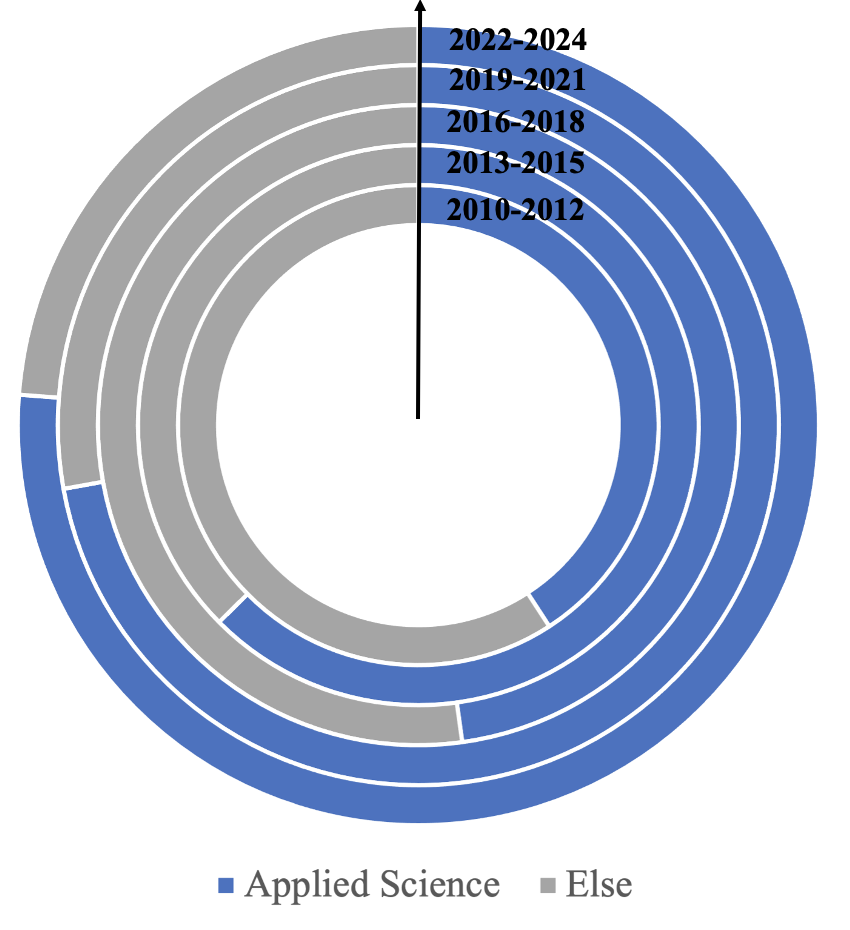
\includegraphics[width=\textwidth]{ProjectReportTemplate/Figures/Applied_Science.png}
      
    \end{minipage}
    \hfill
    \begin{minipage}{0.49\textwidth}
        \centering
        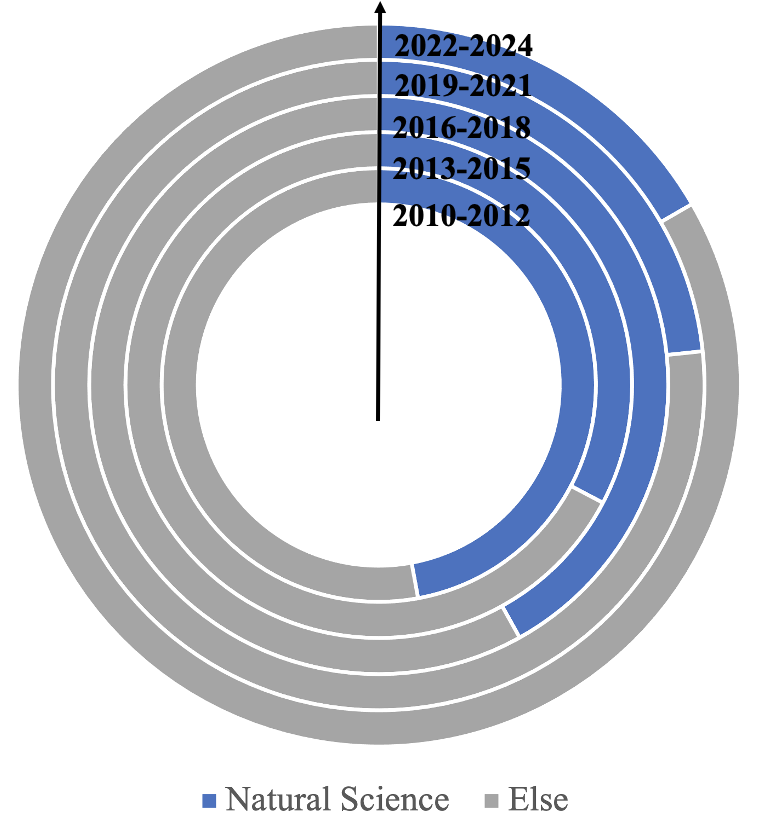
\includegraphics[width=\textwidth]{ProjectReportTemplate/Figures/Natural_Science.png}
       
    \end{minipage}
    
    \begin{minipage}{0.49\textwidth}
        \centering
        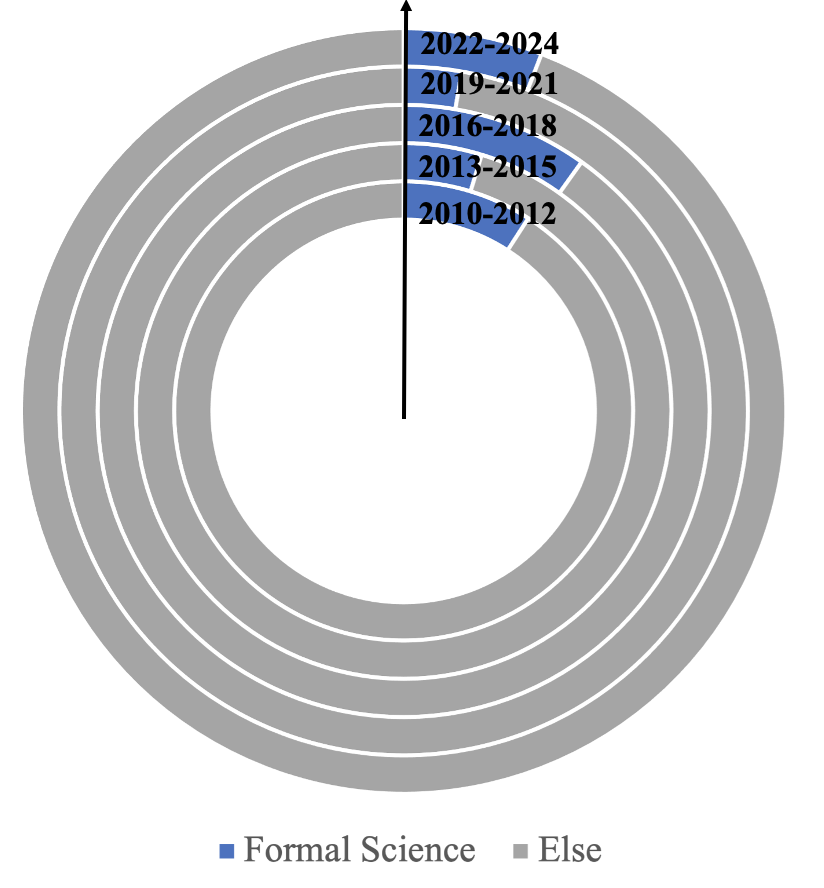
\includegraphics[width=\textwidth]{ProjectReportTemplate/Figures/Formal_Science.png}
    
    \end{minipage}
    \hfill
    \begin{minipage}{0.49\textwidth}
        \centering
        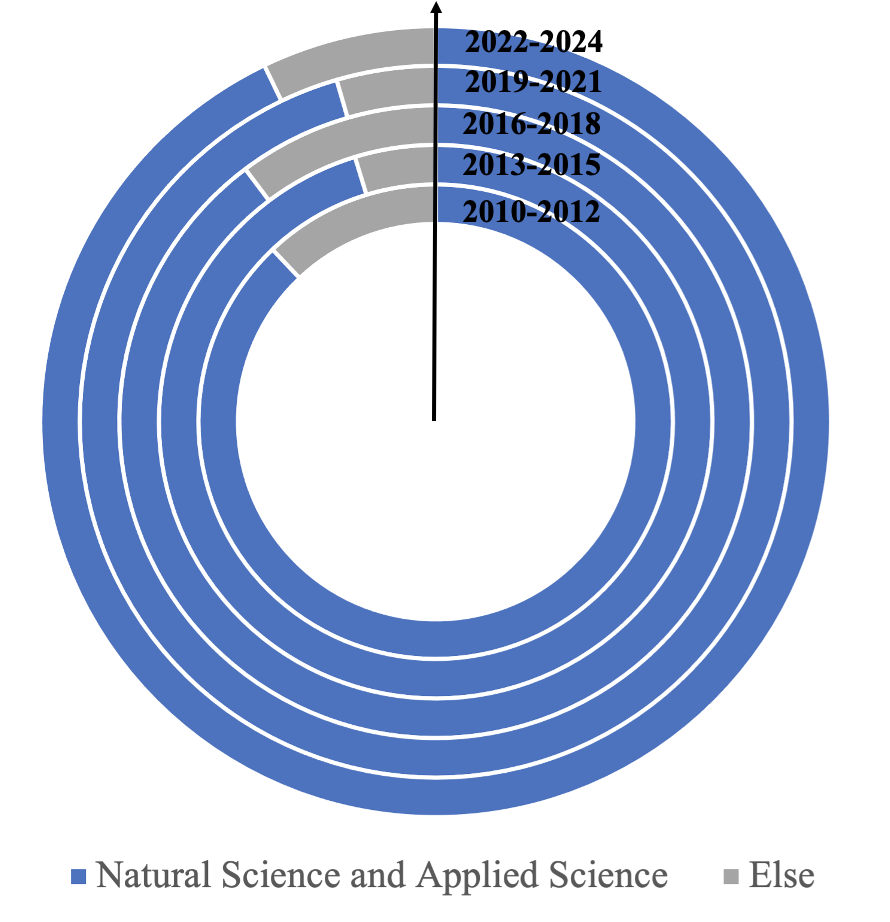
\includegraphics[width=\textwidth]{ProjectReportTemplate/Figures/Applied_Natural_Science.png}
     
    \end{minipage}
    \caption[Proportional Trends Shifting in Research Landscape]{The transition from the inner to the outer circle corresponds to the progression of time from past to present. While the evolution of applied science and natural science exhibits less distinct trends, it is noteworthy that these two domains consistently maintain their status as the most funded areas.}
    \label{fig:combined}
\end{figure}
%TC:endignore


Furthermore, within the realm of social sciences, funding has primarily directed its focus toward public policy. However, the quantity of projects received within the public policy field is comparatively remarkable. Across the periods of 2010-2012, 2019-2021, and 2022-2024, social science has witnessed support solely directed towards public policy. Also, in 2010-2012, 346 projects were funded under the public policy category, surpassing the funding count of any formal science topic and surpassing many themes within the natural science domain. Public policy has emerged as a cornerstone of social science, garnering substantial attention and resources.\\

Moreover, each triennial interval showcases standout topics that have surged ahead and captured substantial funding. For instance, in 2013-2015, "Automotive Engineering" within the Applied Science category witnessed a staggering 1117 funded projects, a testament to its robust prominence. Similarly, 2016-2018 witnessed a surge of funding in the "Material Science" domain, with an impressive tally of 1253 projects. Notably, 2019-2021 witnessed a crescendo in the "Applied Science - Public Health" category, with a significant surge of 1232 funded projects – a phenomenon that perhaps correlates with the emergence of the COVID-19 pandemic.\\

From 2022 to 2024, while Applied Science continues to receive the highest number of funded projects, its subdomains have noticeably decreased. The increase in the overall number of funded projects in Applied Science contrasts with the reduction in the diversity of its subdomains, suggesting a tendency toward consolidation within the Applied Science domain. To be specific, 68.75\% of the investment directions in applied science for 2022-2024 align with those invested during 2019-2021.\\

%TC:ignore
\begin{figure}[H]
    \centering
    \begin{minipage}{0.7\textwidth}
        \centering
        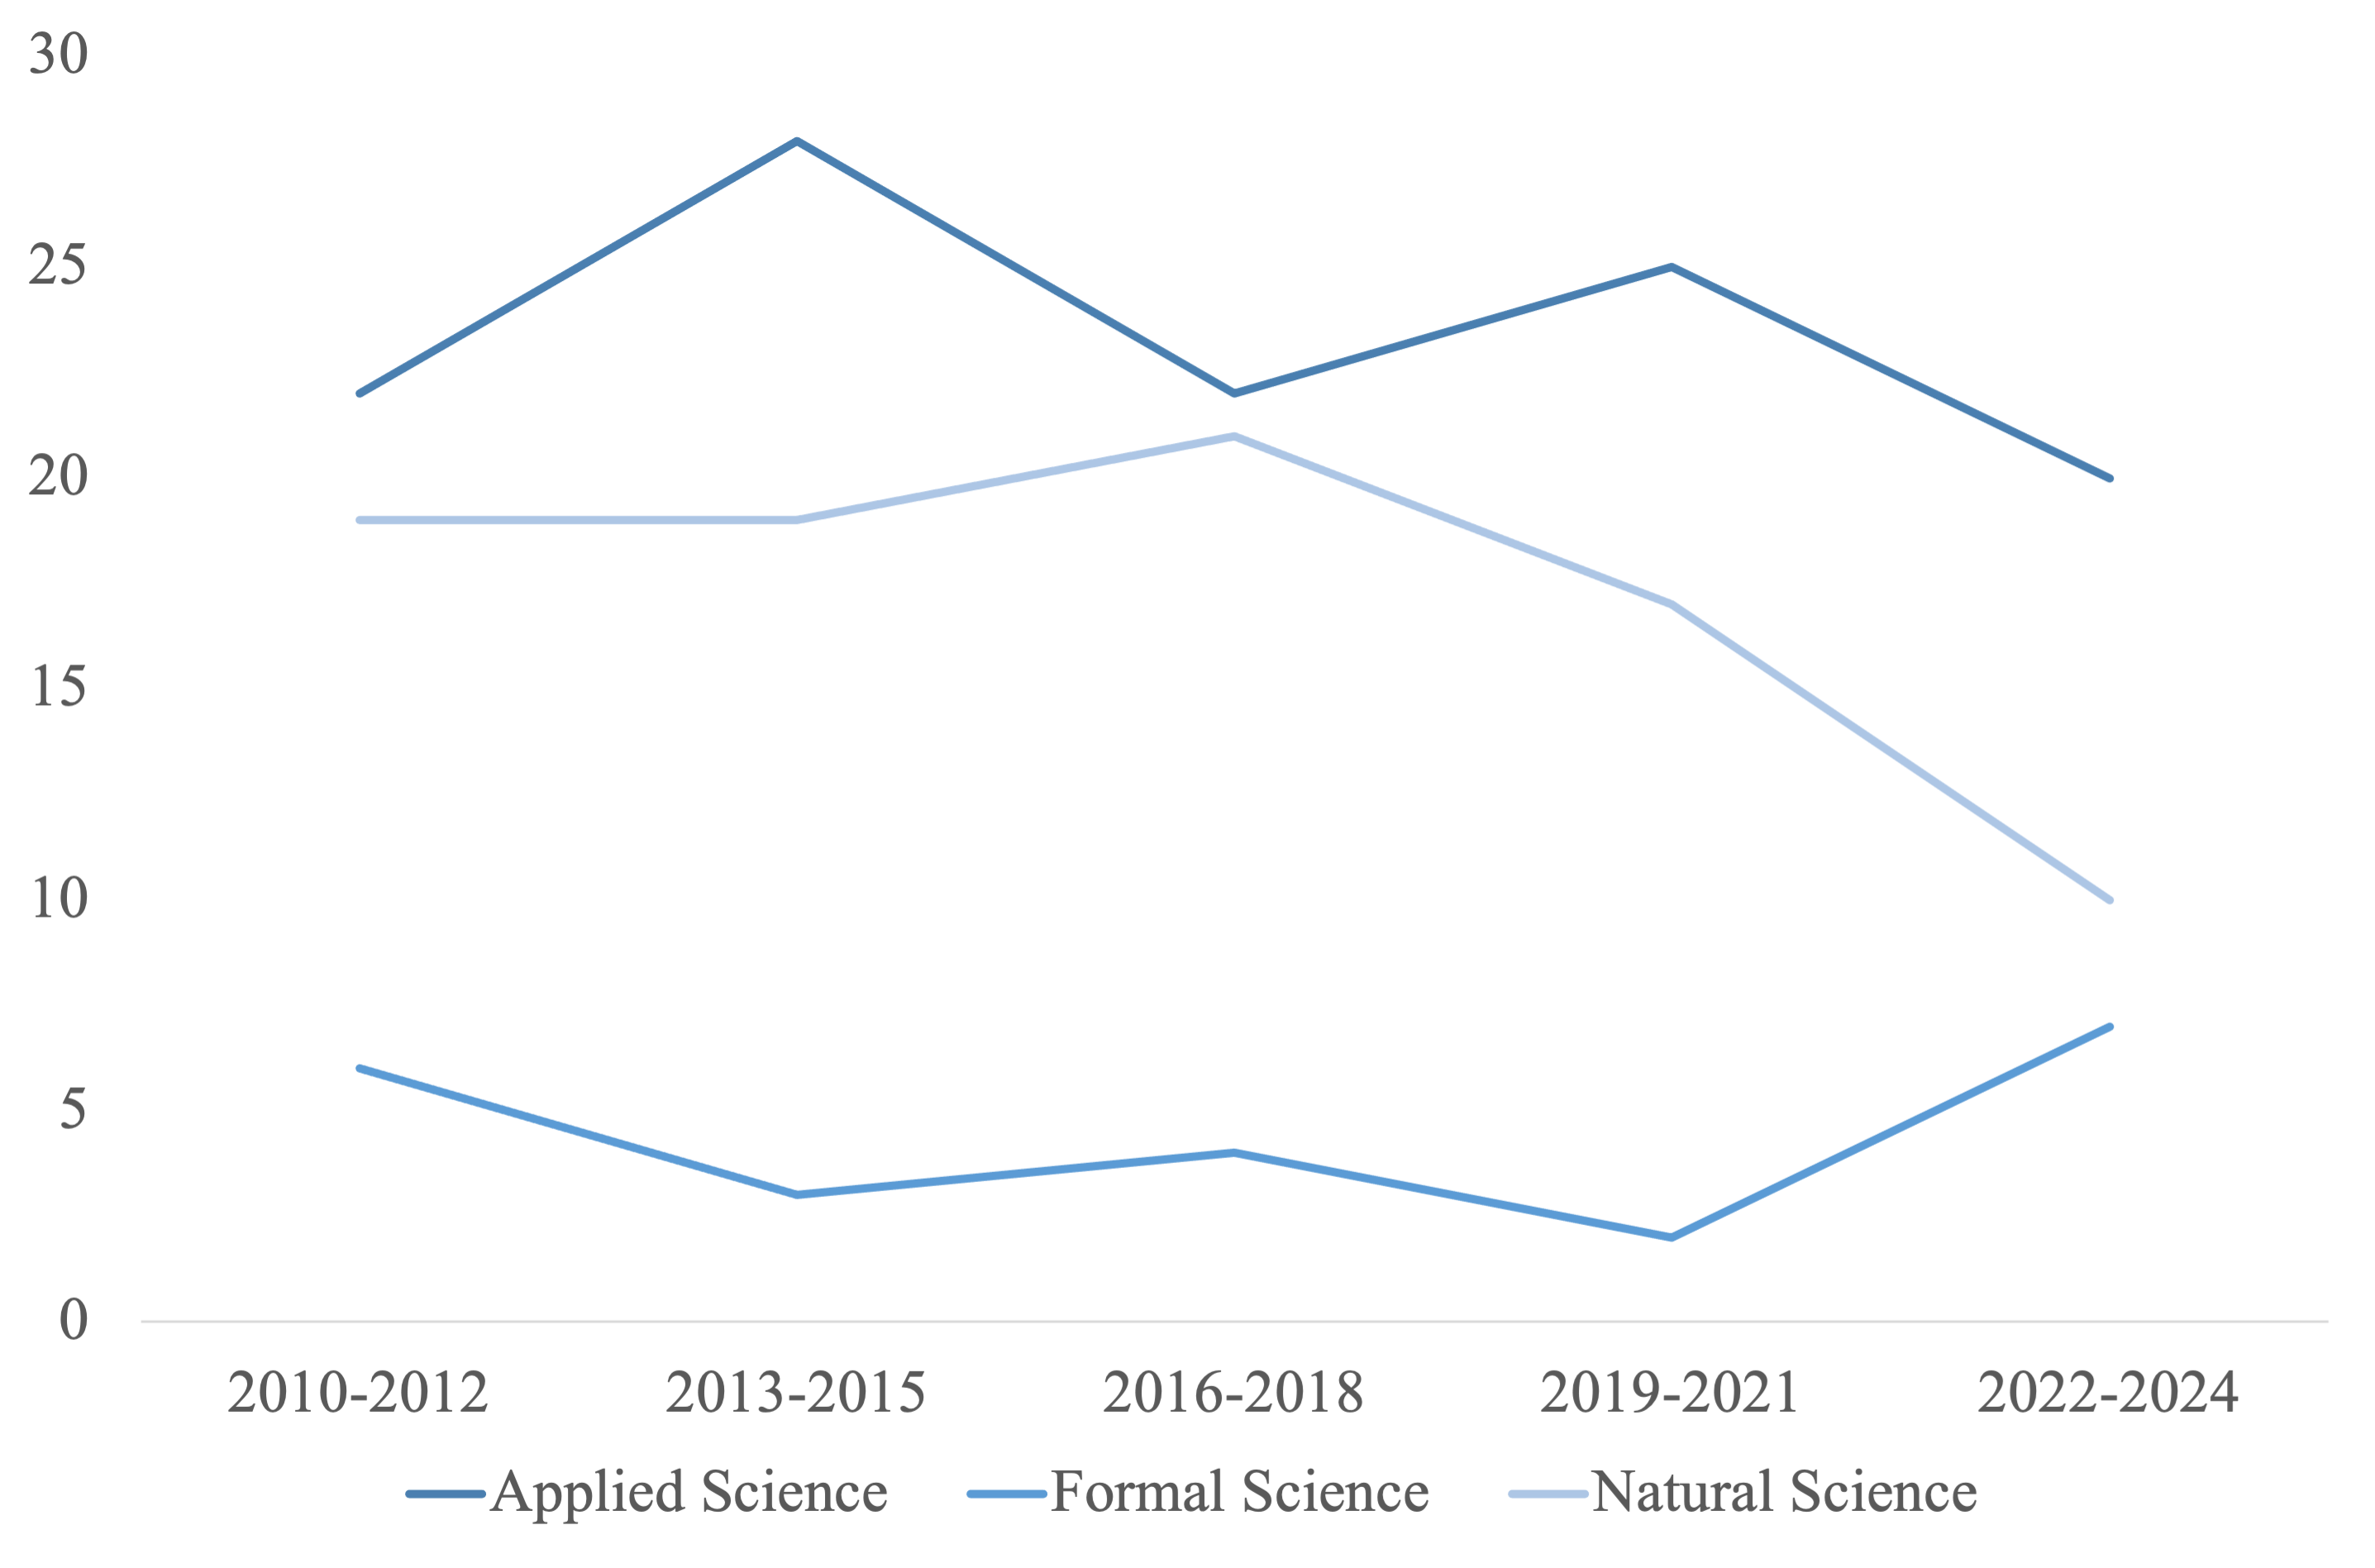
\includegraphics[width=\textwidth]{Figures/The number of subdomains within each category.png}
      
    \end{minipage}

    \begin{minipage}{0.7\textwidth}
        \centering
        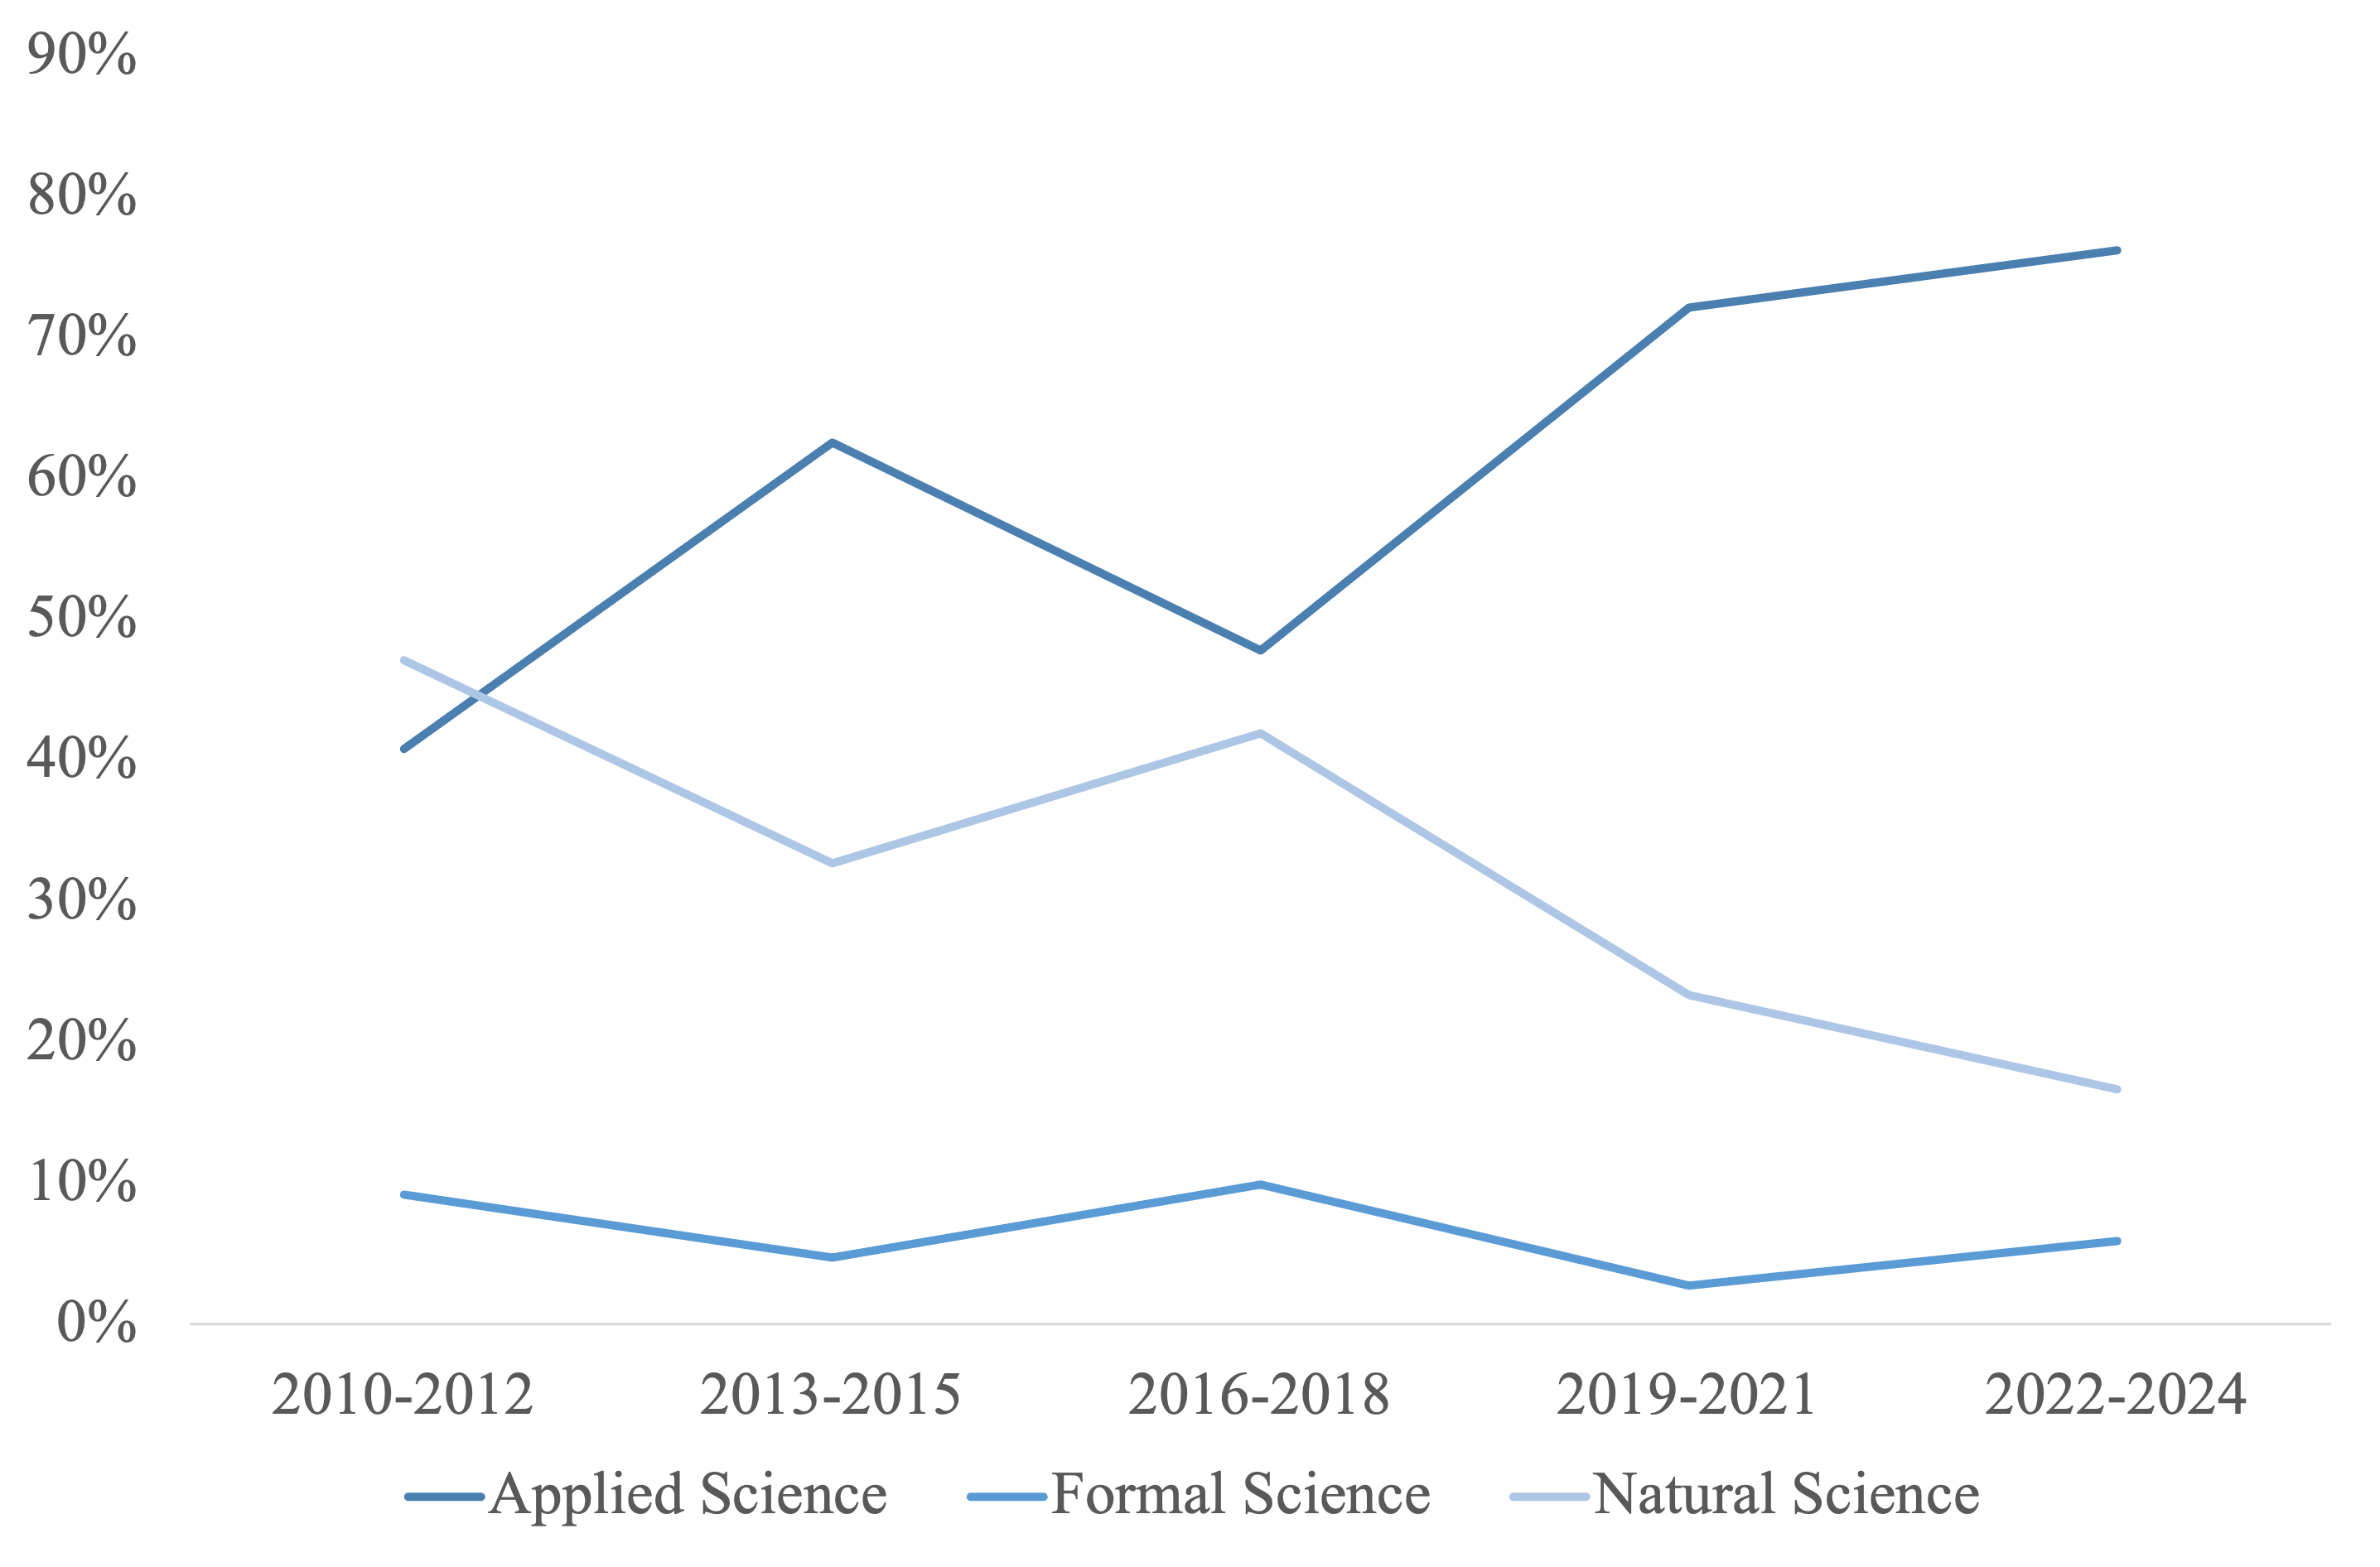
\includegraphics[width=\textwidth]{Figures/Evolution of Funding Distribution Across Categories.png}
       
    \end{minipage}
 
    \caption[Changing Subdomain Counts Across Categories Over Time]{
The upper figure showcases shifts in the count of funded subdomains within each category. The lower figure portrays the ratio of the number of funded subdomains normalized by the total project count.}
    \label{fig:combined}
\end{figure}
%TC:endignore
Despite minor fluctuations in the proportional distribution of project counts across various categories, a consistent trend emerges over the 21-year period. Applied Science and Natural Science have consistently maintained a notable advantage, collectively accounting for over half of the funded projects. Formal Science, particularly Mathematics and Statistics as foundational disciplines, have exhibited a consistent presence with a smaller yet stable number of funded projects. In contrast, Social Science received minimal funding during 2013-2015, rendering its contribution negligible and thus not represented on the line graph for visual clarity.\\


Funding for Applied Science projects shows an overall upward trend, whereas Natural Science projects exhibit an overall downward trend, and Formal Science projects maintain relatively stable funding allocation. Hence, it can be inferred that Applied Science has, to a certain extent, encroached upon the funding allocation that might have originally been directed toward Natural Science.\\

The number of subdomains within Applied Science and Natural Science has notably decreased, indicating a trend toward consolidation in both domains. I have created a heatmap for detailed analysis to gain more insight into these subdomain dynamics.\\

In comparison to the period between 2019 and 2021, a significant influx of funding in the realm of natural sciences has been directed toward environmental and material science from 2022 to 2024. However, no prominent research directions have been identified within applied science.
%TC:ignore
\begin{figure}[H]
    \centering
    \begin{minipage}{\textwidth}
        \centering
        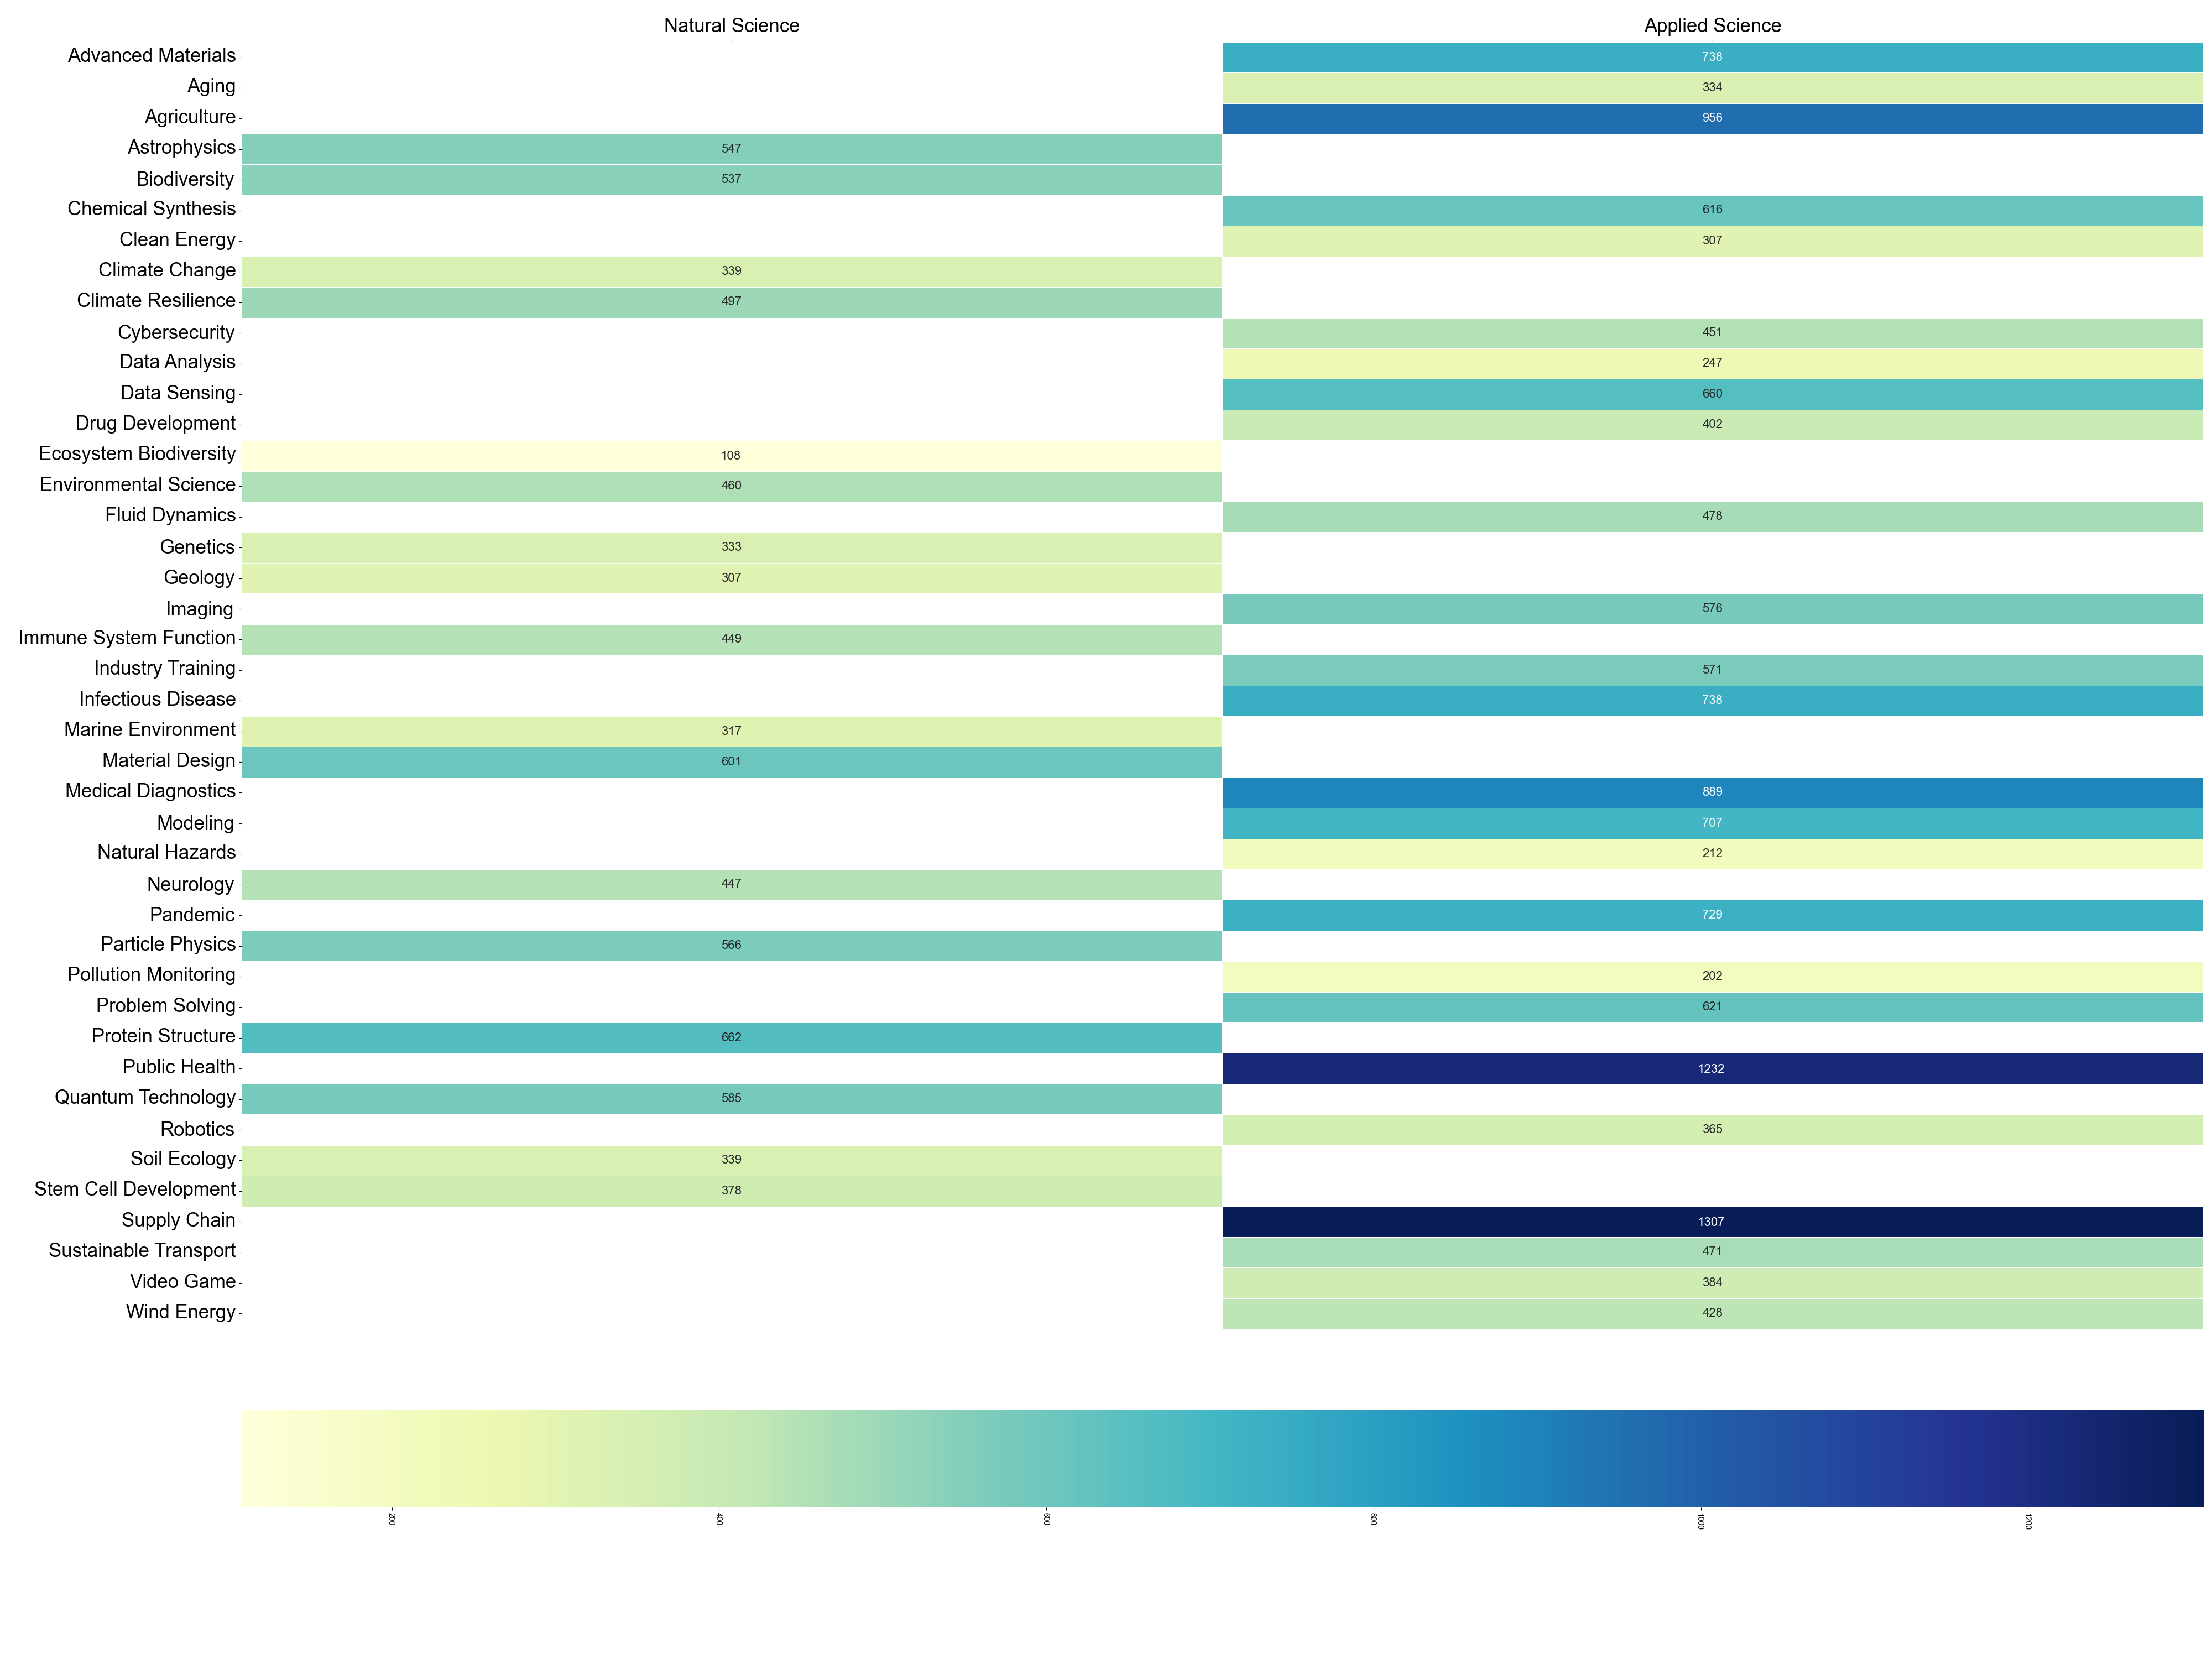
\includegraphics[width=0.95\textwidth]{ProjectReportTemplate/Figures/2019_2021_heatmap.png}
      
    \end{minipage}

    \begin{minipage}{\textwidth}
        \centering
        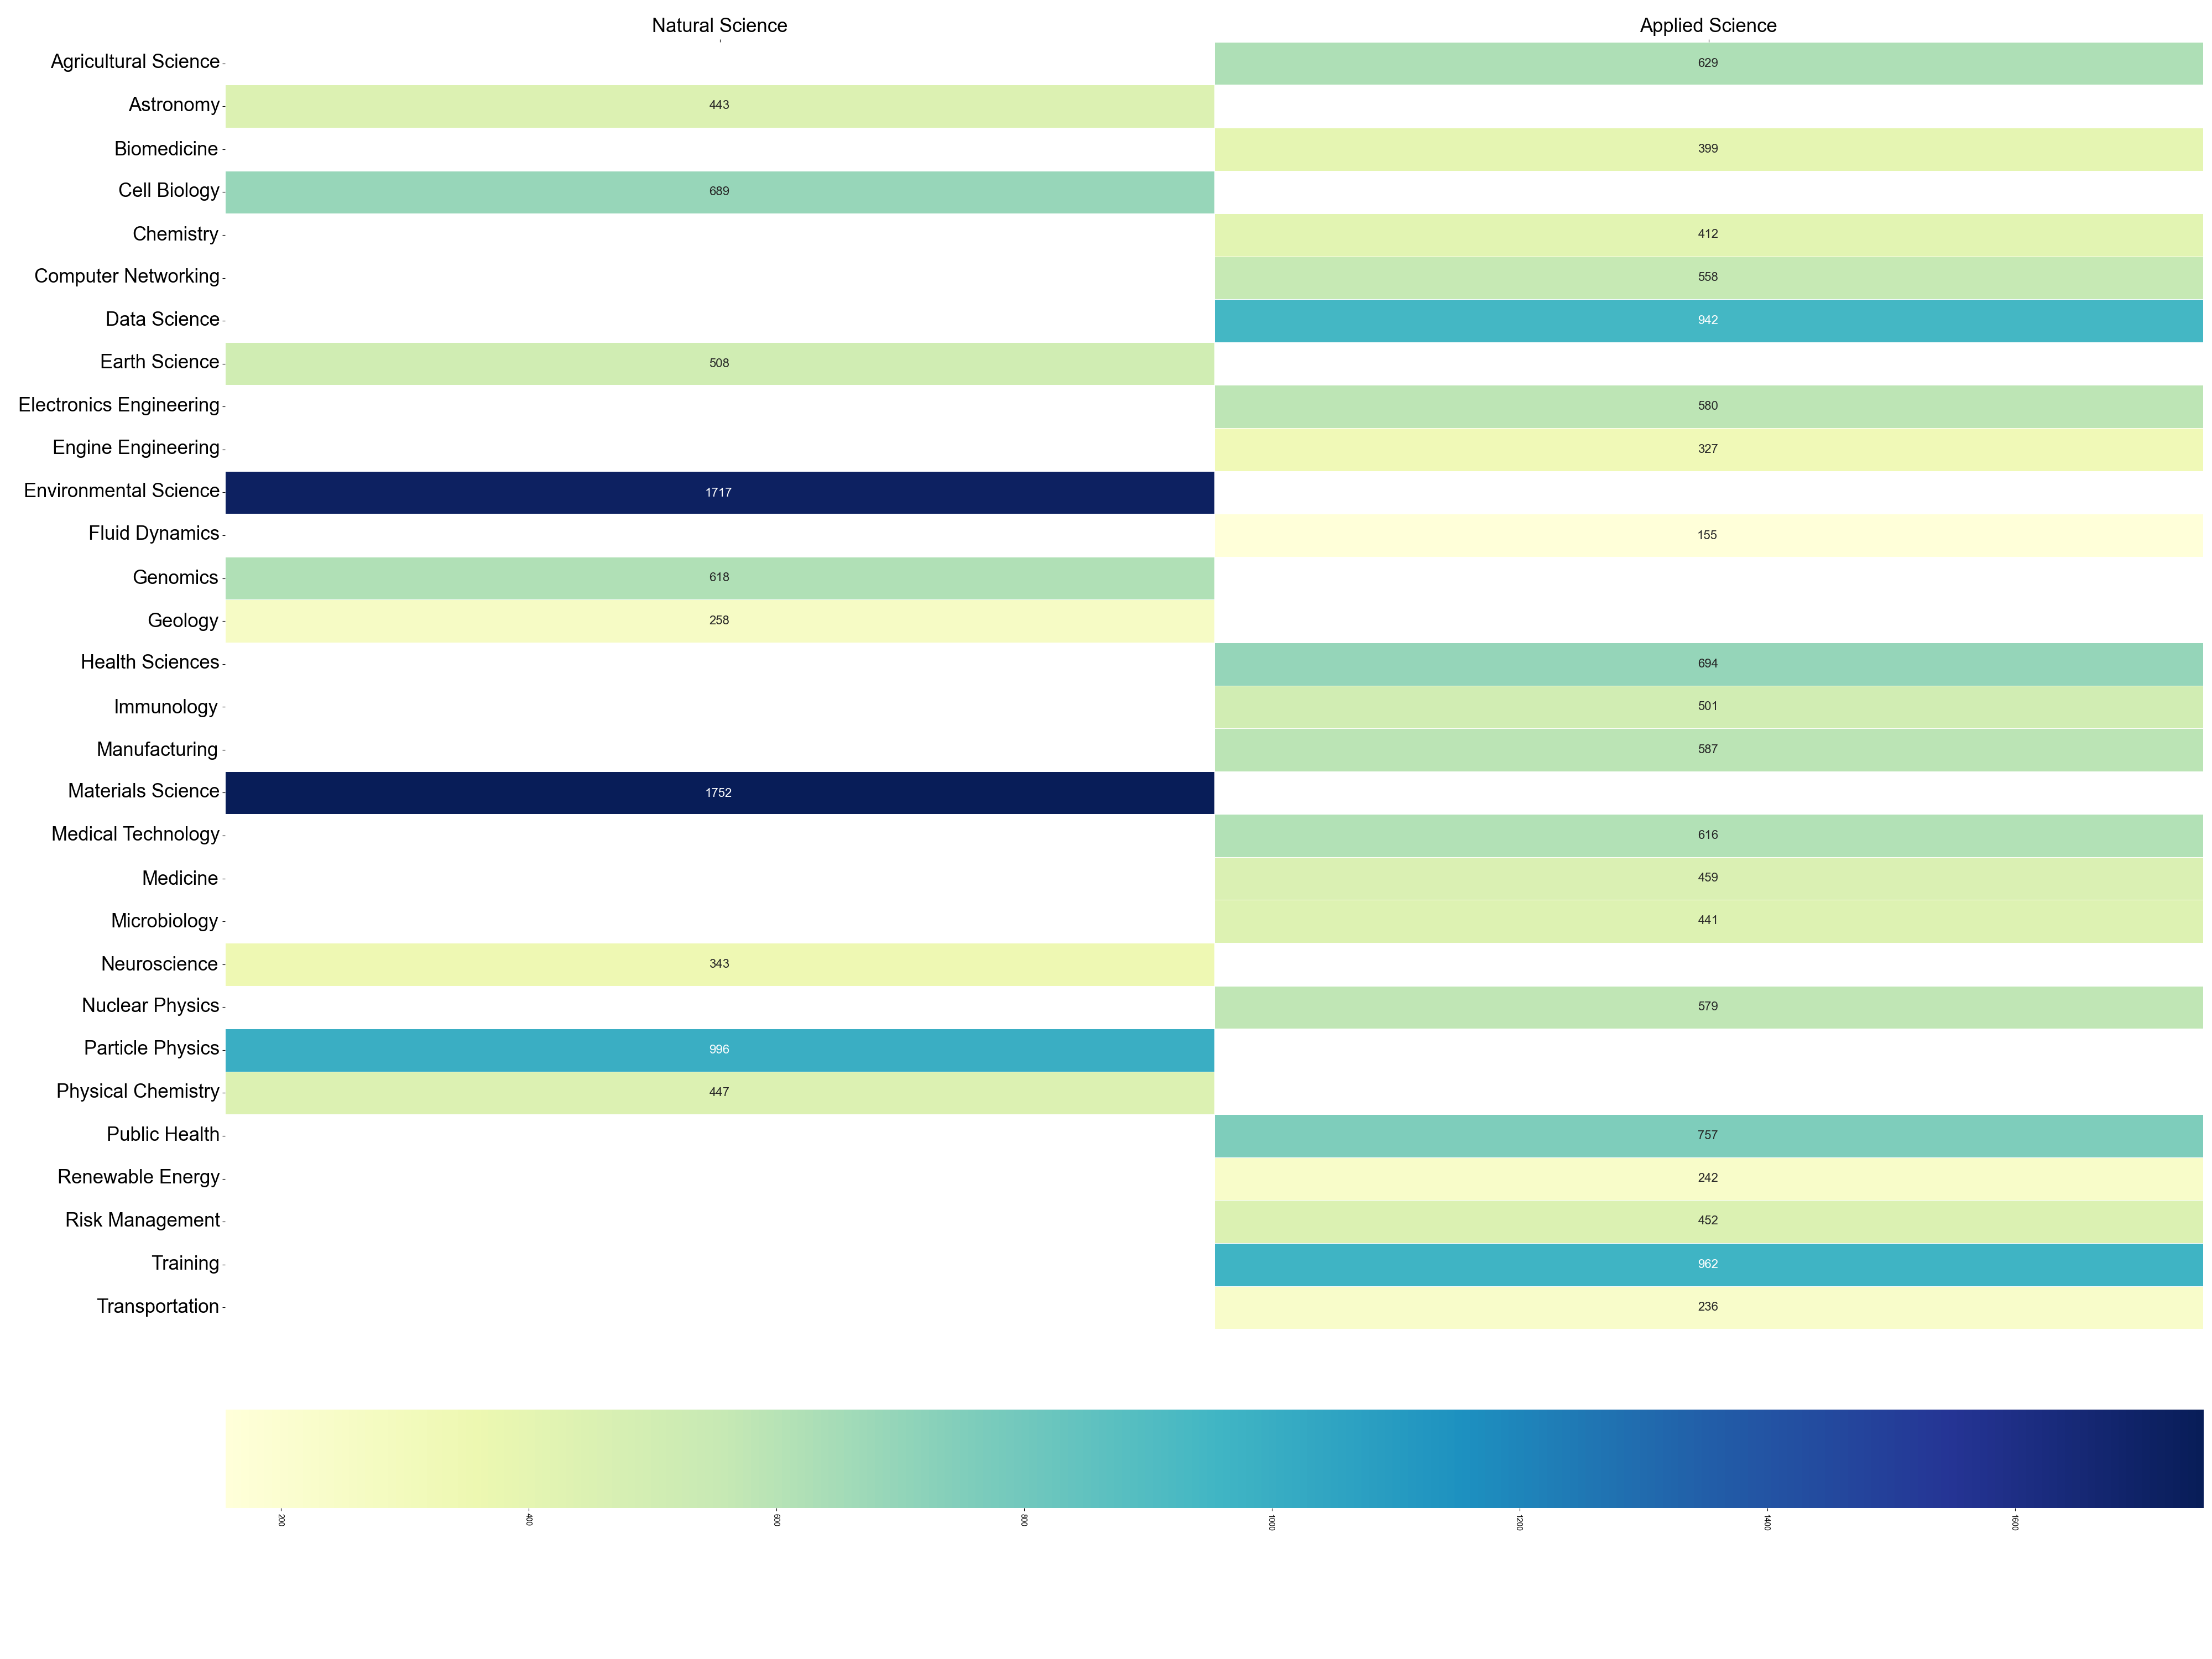
\includegraphics[width=0.95\textwidth]{ProjectReportTemplate/Figures/2022_2024_heatmap.png}
       
    \end{minipage}
 
    \caption[Project Counts distribution of Applied Science and Natural Science]{A huge amount of funding is directed towards Environmental Science and Materials Science.}
    \label{fig:combined}
\end{figure}
%TC:endignore


An aspect worthy of attention is the sustained inclusion of ecology within the funded projects list, maintaining a prominent position throughout each three-year interval. 
%TC:ignore
\begin{figure}[H]
\centering
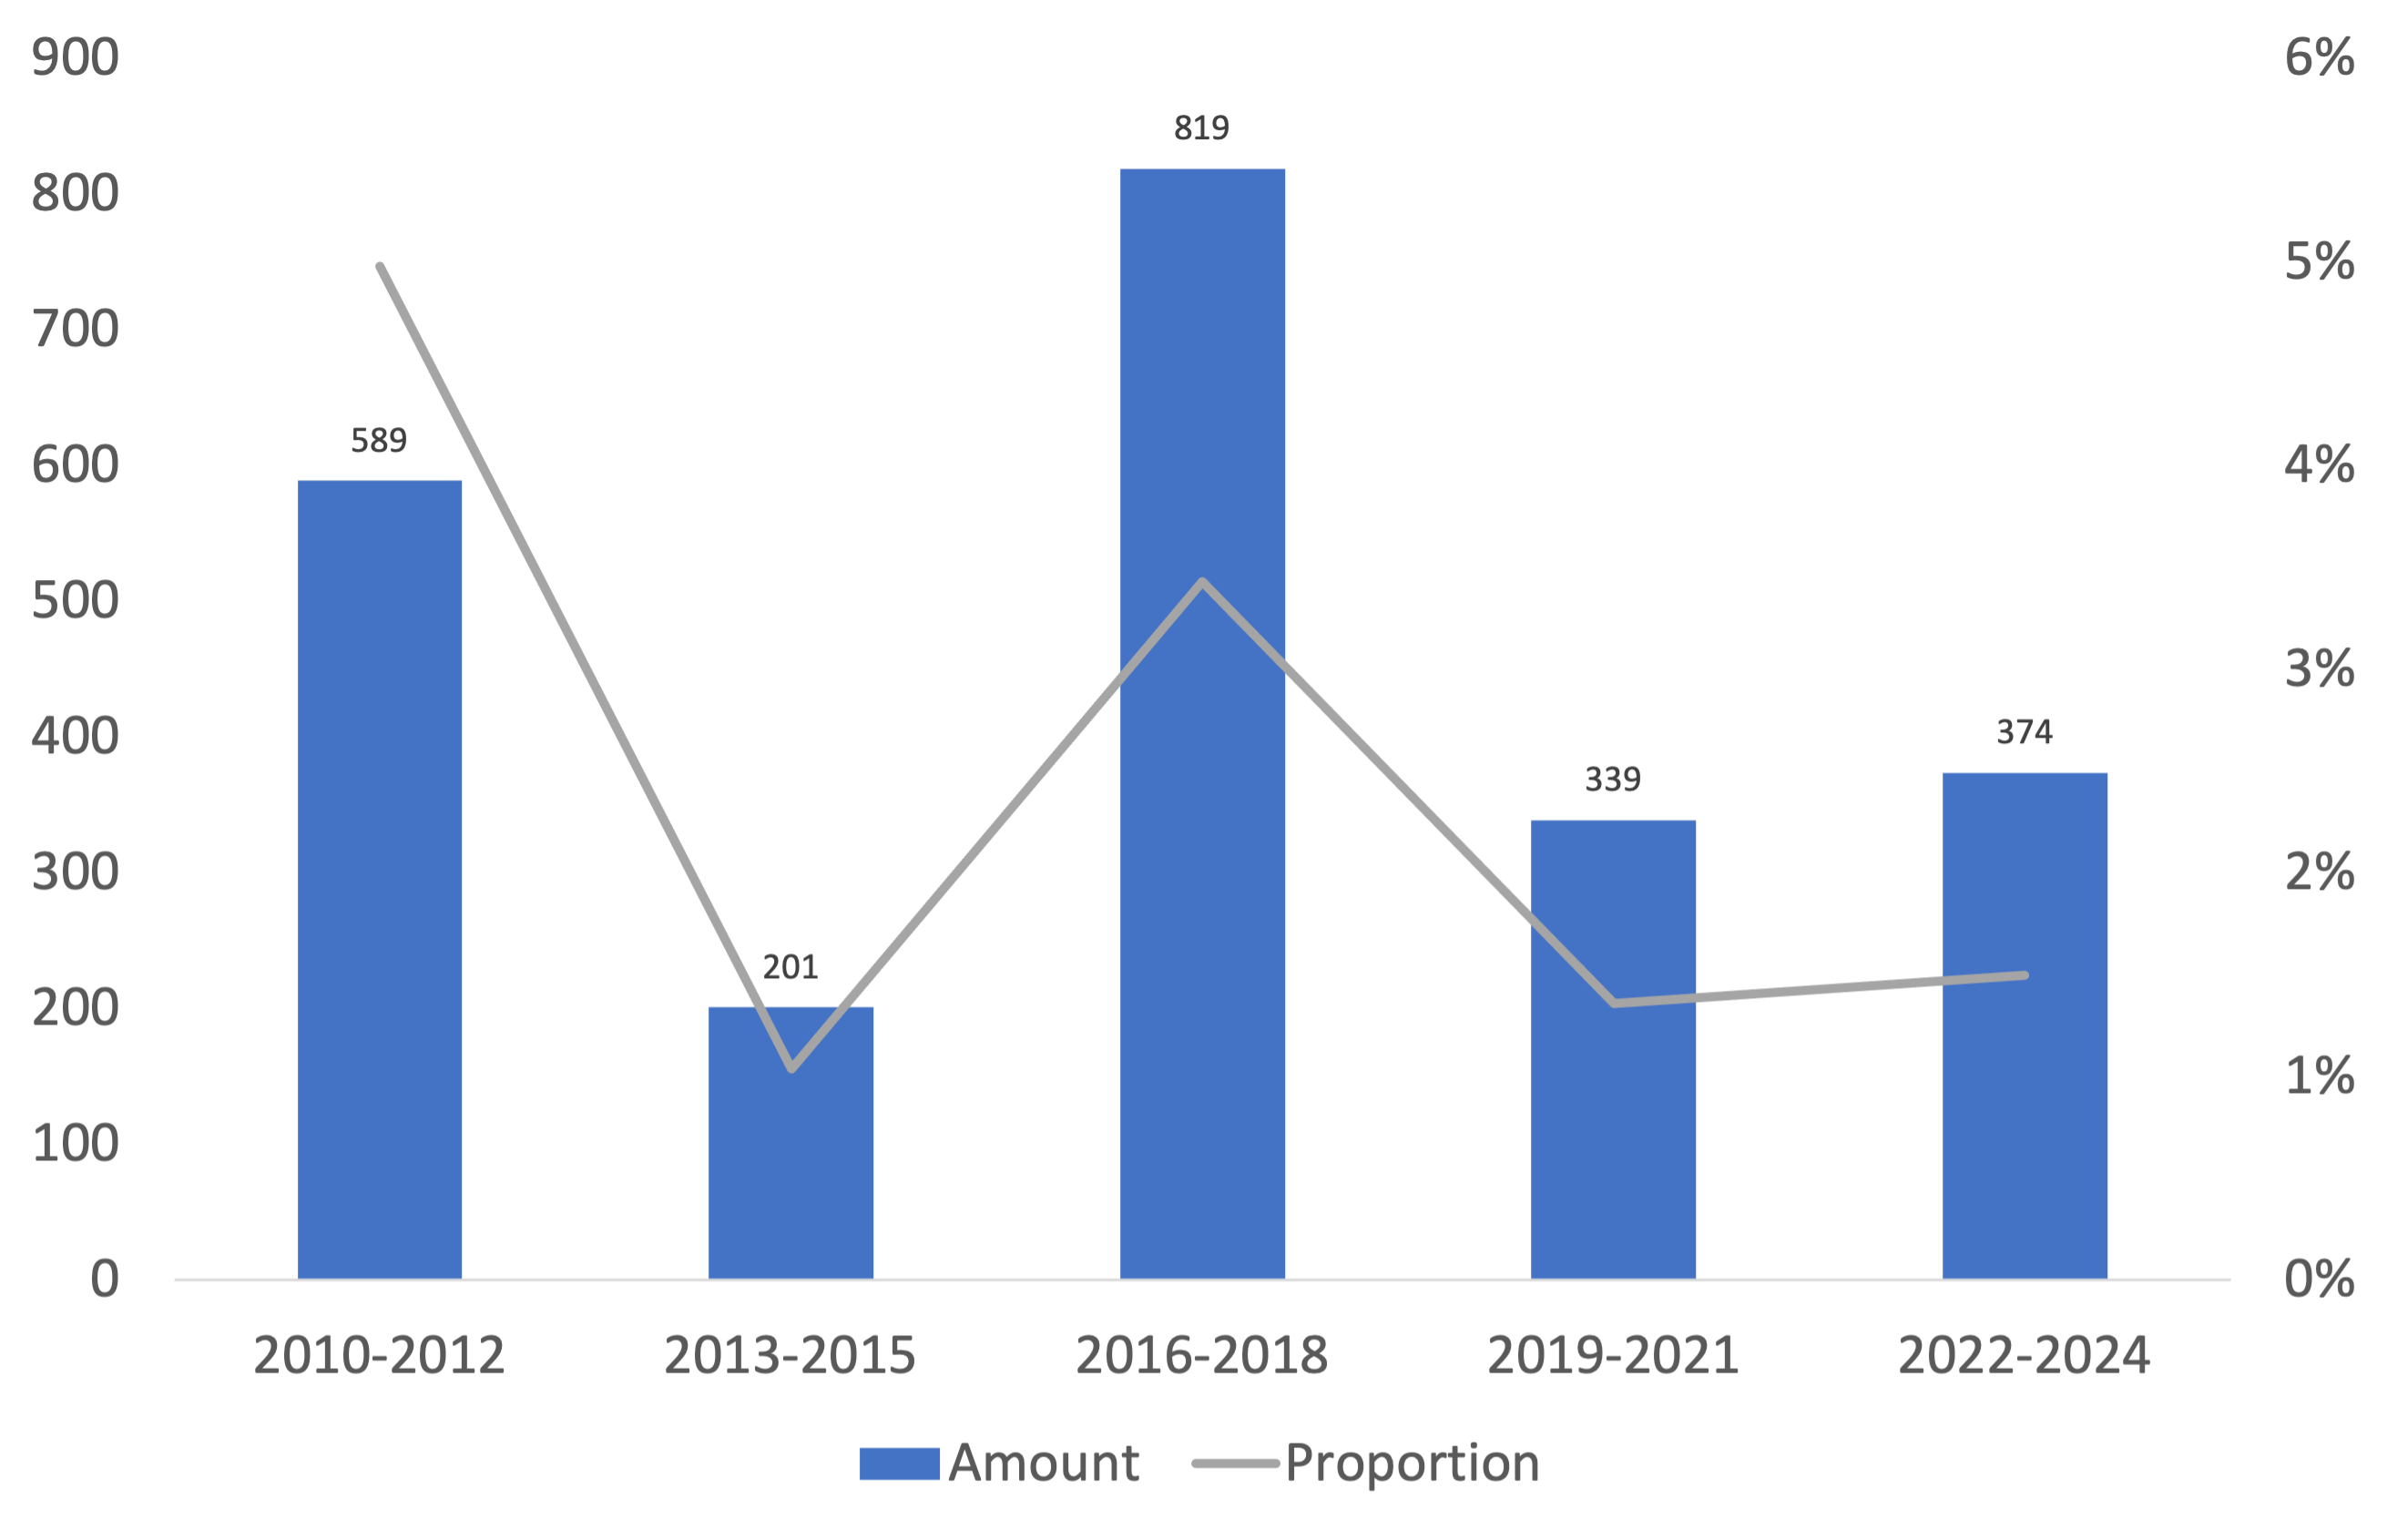
\includegraphics[scale=0.7]{Figures/Landscape of Ecology Funding.png}
\caption[Changing Landscape of Ecology Funding]{Ecology has consistently secured funding for several hundred projects during each triennial period.}
\label{figure} 
\end{figure}
%TC:endignore
In contrast, evolutionary biology has not received funding at a high frequency, with only 203 projects receiving funding between 2010 and 2012. Subsequently, the number of funded projects related to this field has remained notably low across the entire dataset.

\section*{Overall Analysis Based on Funding Amount}

In addition to project count, the amount of funding allocated to projects in different domains can also indicate the level of attention and popularity within each respective field. The funding received by projects across various domains reflects the extent of emphasis and interest dedicated to those domains, thereby providing valuable insights into their prominence and significance.\\

Over the past two decades, there has been a noticeable upward trend in the funding amounts provided by UKRI. Specifically, the funding amounts for the periods 2010-2012, 2013-2015, 2016-2018, 2019-2021, and 2022-2024 have been £3,150,014,803, £5,859,873,507, £7,314,254,625, £7,507,960,726, and £7,285,275,813, respectively. It is important to emphasize that the funding amount for 2022-2024 is based on data up to 2022 rather than being the most up-to-date information. Consequently, a substantial number of projects have not yet been included in the analyzed data, resulting in a seemingly reduced figure. Furthermore, numerous projects are still in the application phase, including cases like the "Knowledge transfer partnerships (KTP): 2023 to 2024 round four," where the allocation of the £9,000,000 funding remains pending.\\


UKRI continues to invest more in "applied science" and "natural science." While the proportions of these two categories of projects have changed over time, their combined total has consistently remained above 80\%. Notably, during 2013-2015 and 2016-2018, this proportion reached an astonishing 96\%. This trend highlights the significant importance UKRI places on these areas and underscores the greater need for research funding for projects within these domains. It also indicates that, to a certain extent, they have reallocated funding from other category projects.\\

%TC:ignore
\begin{figure}[H]
\centering
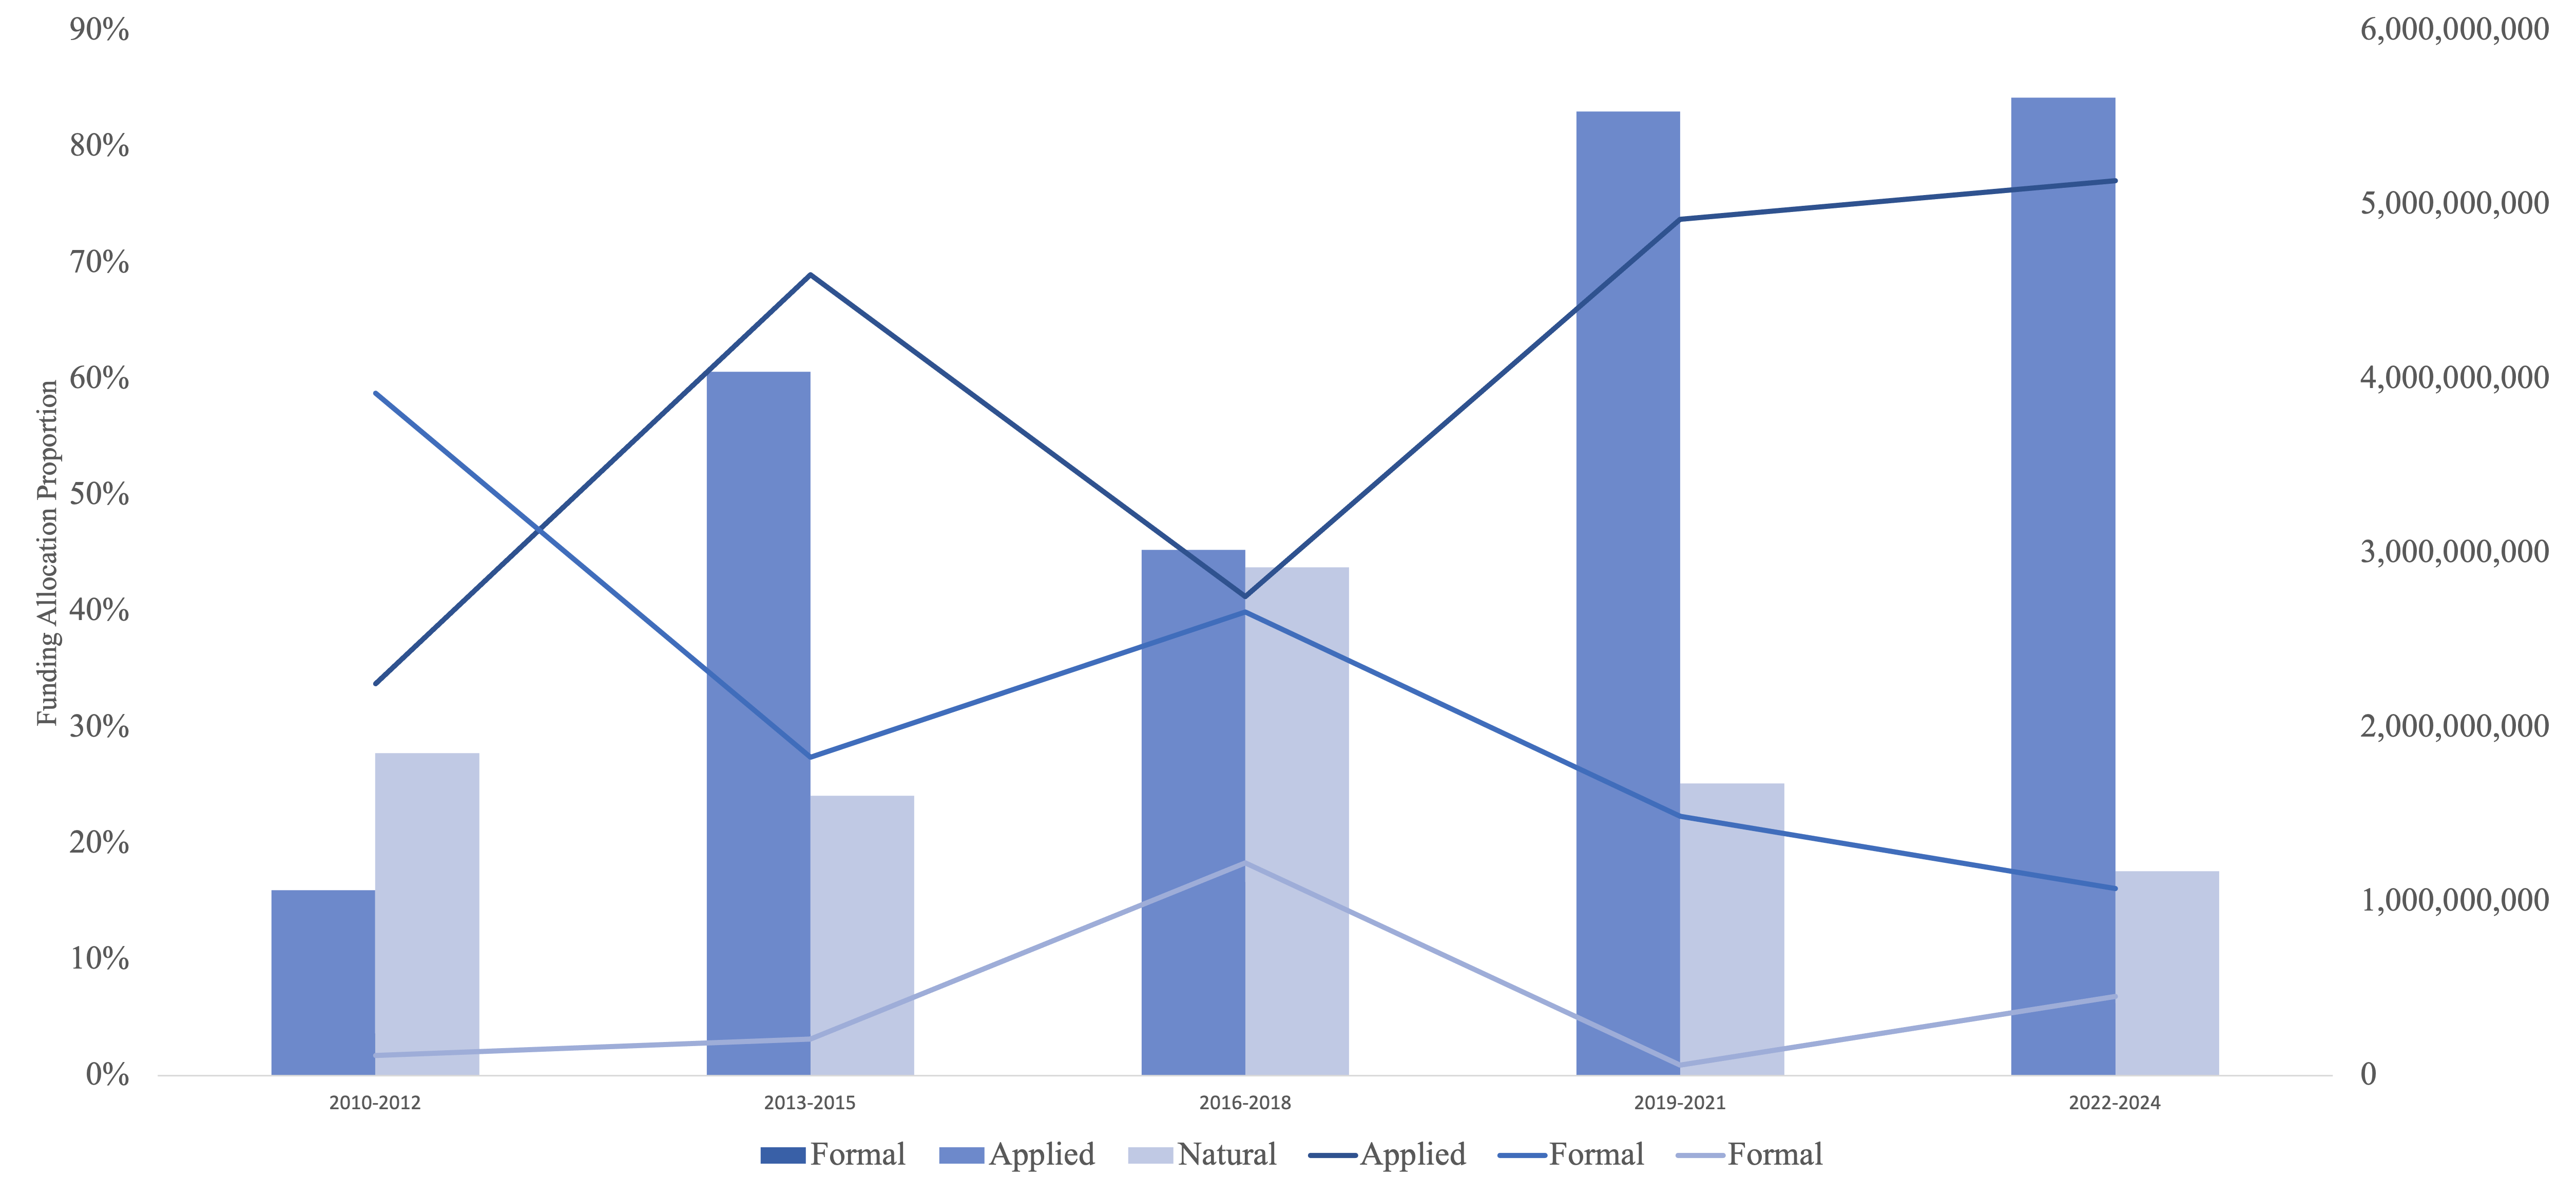
\includegraphics[scale=0.4]{Figures/funding_amount.png}
\caption[Evolution of Funding Trends Across Categories]{Applied Science continues to exhibit an upward trajectory in funding amounts, maintaining the highest proportion of funding allocation.}
\label{figure3.5} 
\end{figure}
%TC:endignore
Upon closer examination of each three-year interval, in each interval, UKRI's focus within the natural sciences field has continuously evolved. For instance, From 2013 to 2015, UKRI allocated substantial funding towards Energy Systems and Technology Innovation, providing support amounting to £512,227,820 and £406,407,200, respectively. However, of even greater significance is UKRI's evident keenness towards the health and longevity of humanity. Cell Biology received a substantial grant of £48,791,642, while Aging research secured £310,492,126, and Public Health initiatives were granted £185,898,579. Further, considerable support was extended to Medical Technology with £83,056,741 in funding, and Cardiovascular Diseases research obtained £65,710,644, among numerous other related projects. This demonstrates UKRI's concerted efforts to drive advancements in diverse fields critical to human well-being.\\

However, a notable shift in focus occurred during 2016-2018, as UKRI redirected its attention towards environmental concerns. During this period, natural science topics that received the highest funding included Energy Systems with £112,236,139 and Environmental Pollution with £358,116,908, encompassing Earth Science with a funding allocation of £163,914,390. This phase witnessed a substantial increase in funding for numerous environmental protection and sustainability initiatives. Similarly, in the subsequent interval of 2019-2021, UKRI continued this trend by allocating £127,302,749 to Wind Energy, £94,358,531 to Clean Energy, and a substantial £155,449,671 to Marine Environment projects.\\


%TC:ignore
\begin{figure}[H]
    \centering

    \begin{subfigure}{\textwidth}
        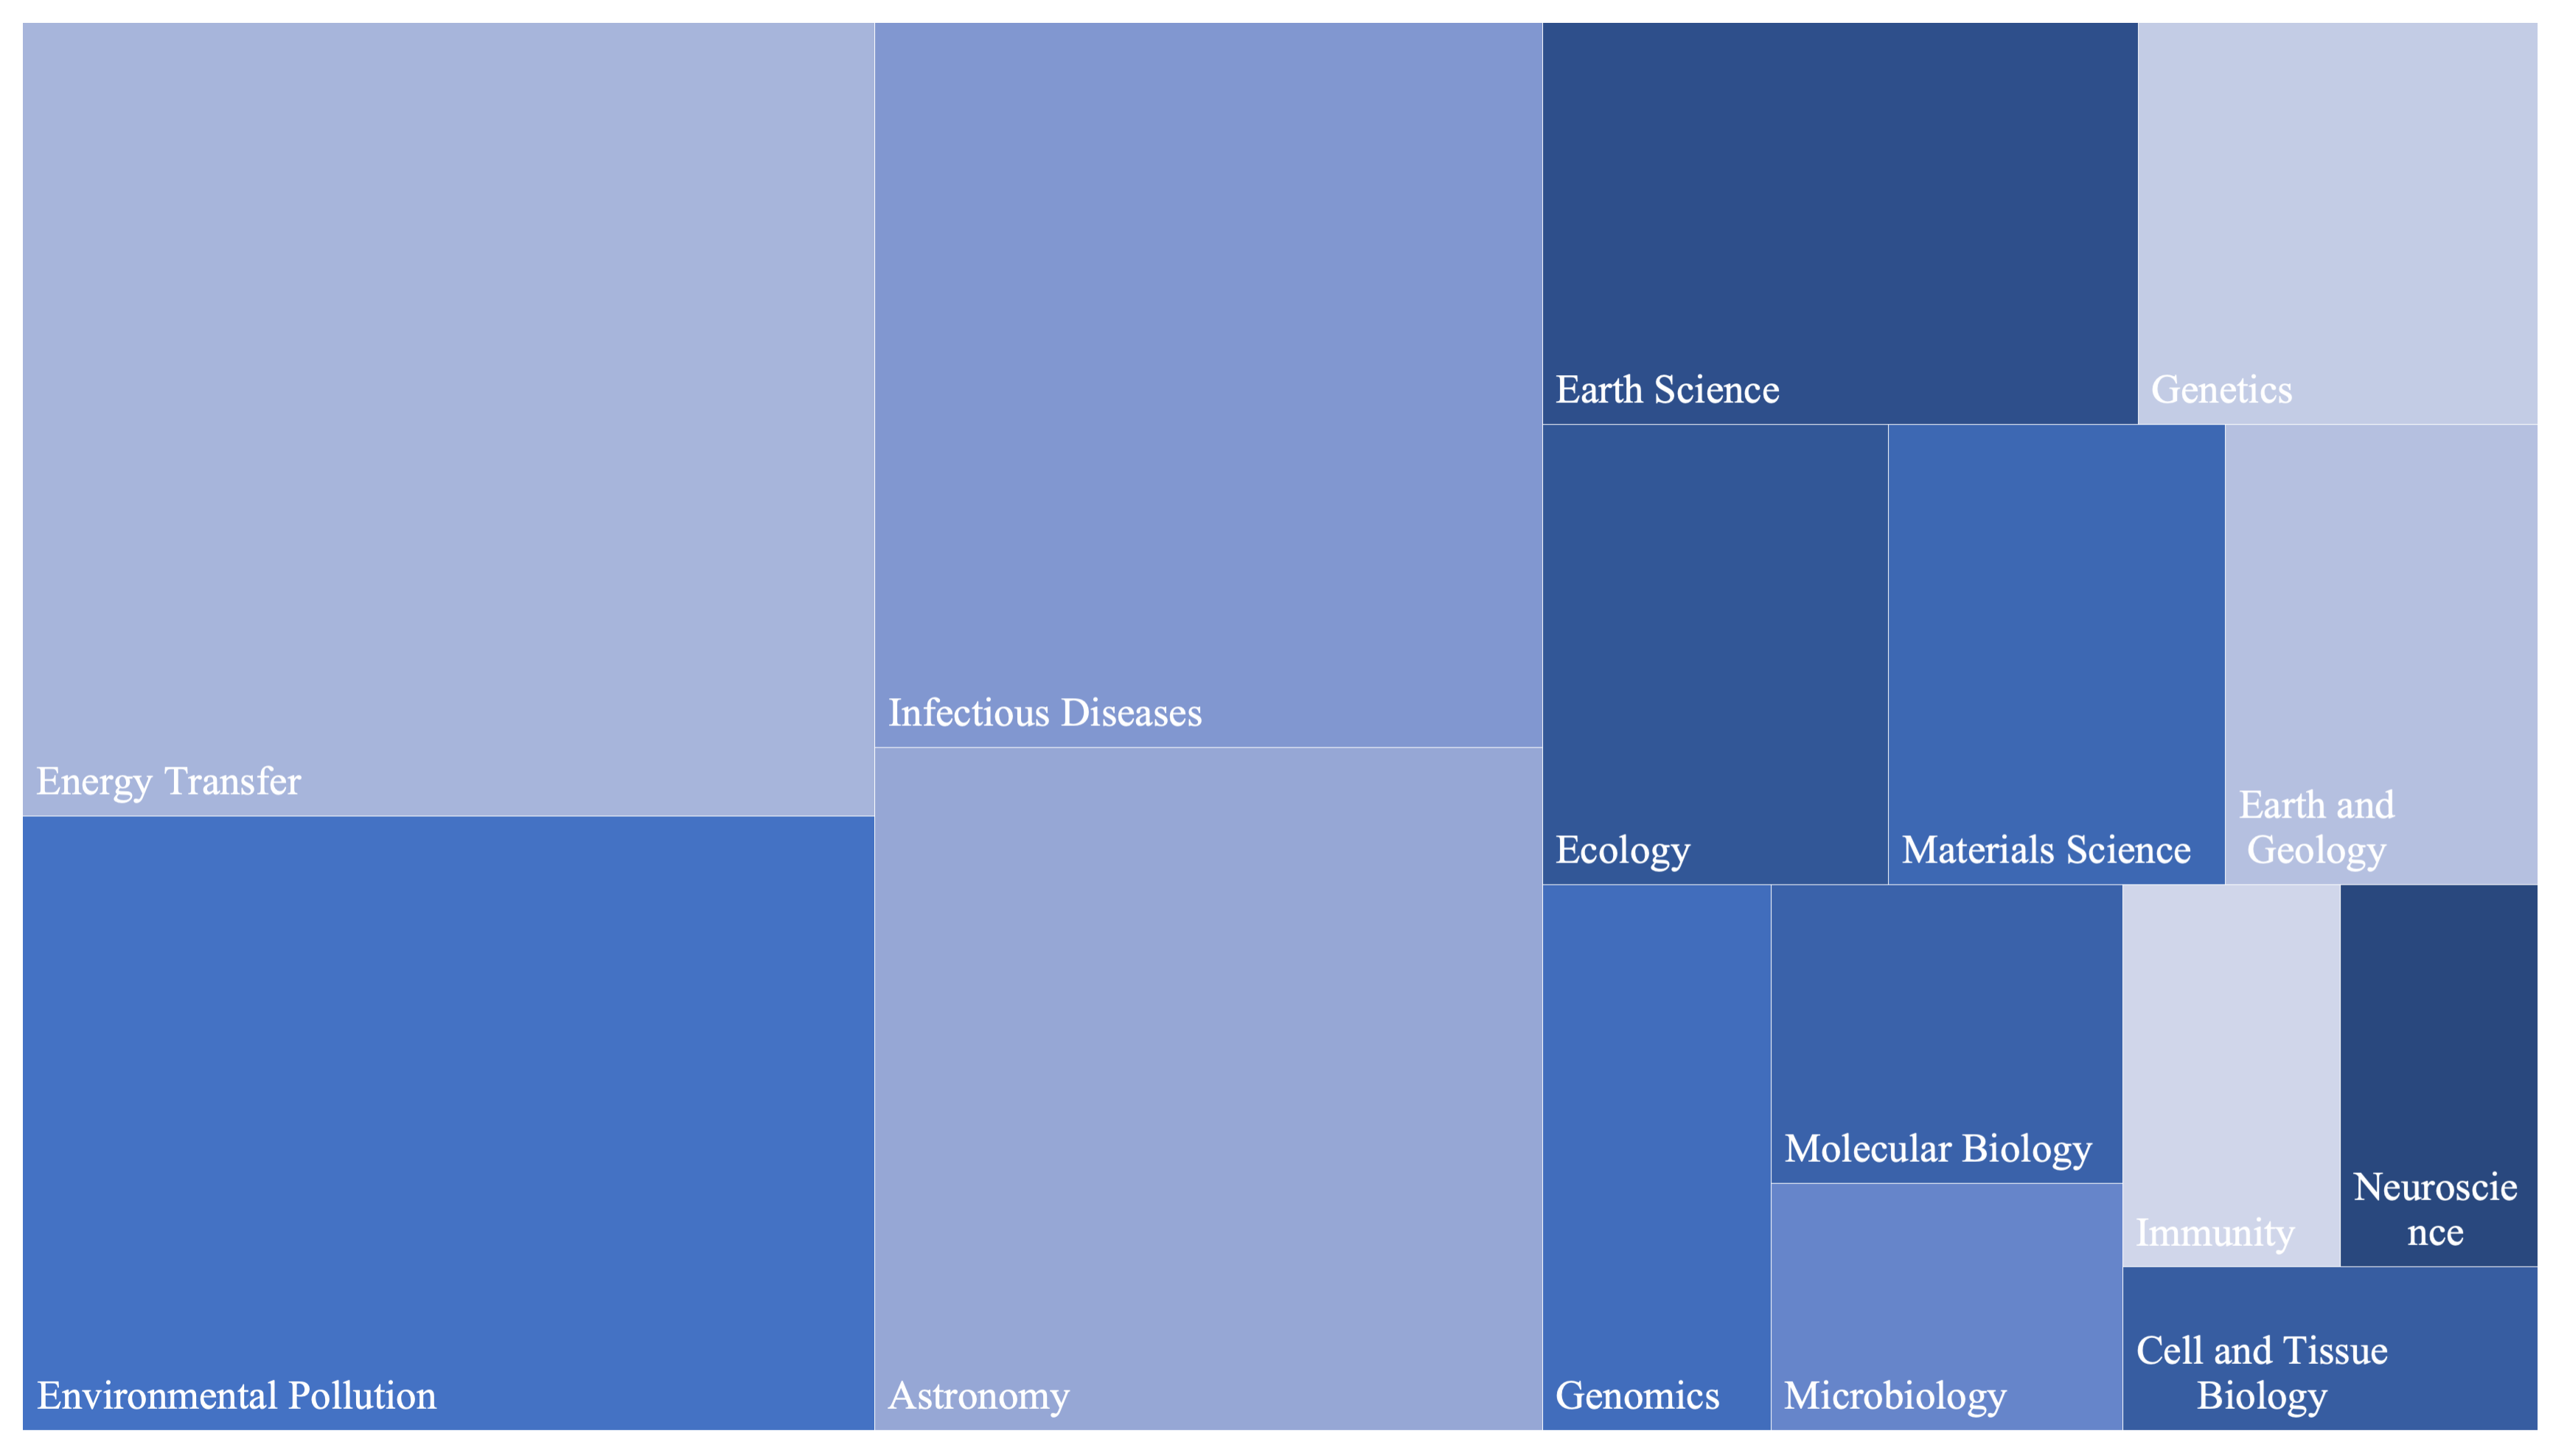
\includegraphics[width=\textwidth]{Figures/Overview of Natural Science Projects Funded in 2016-2018.png}

    \end{subfigure}
    \begin{subfigure}{\textwidth}
        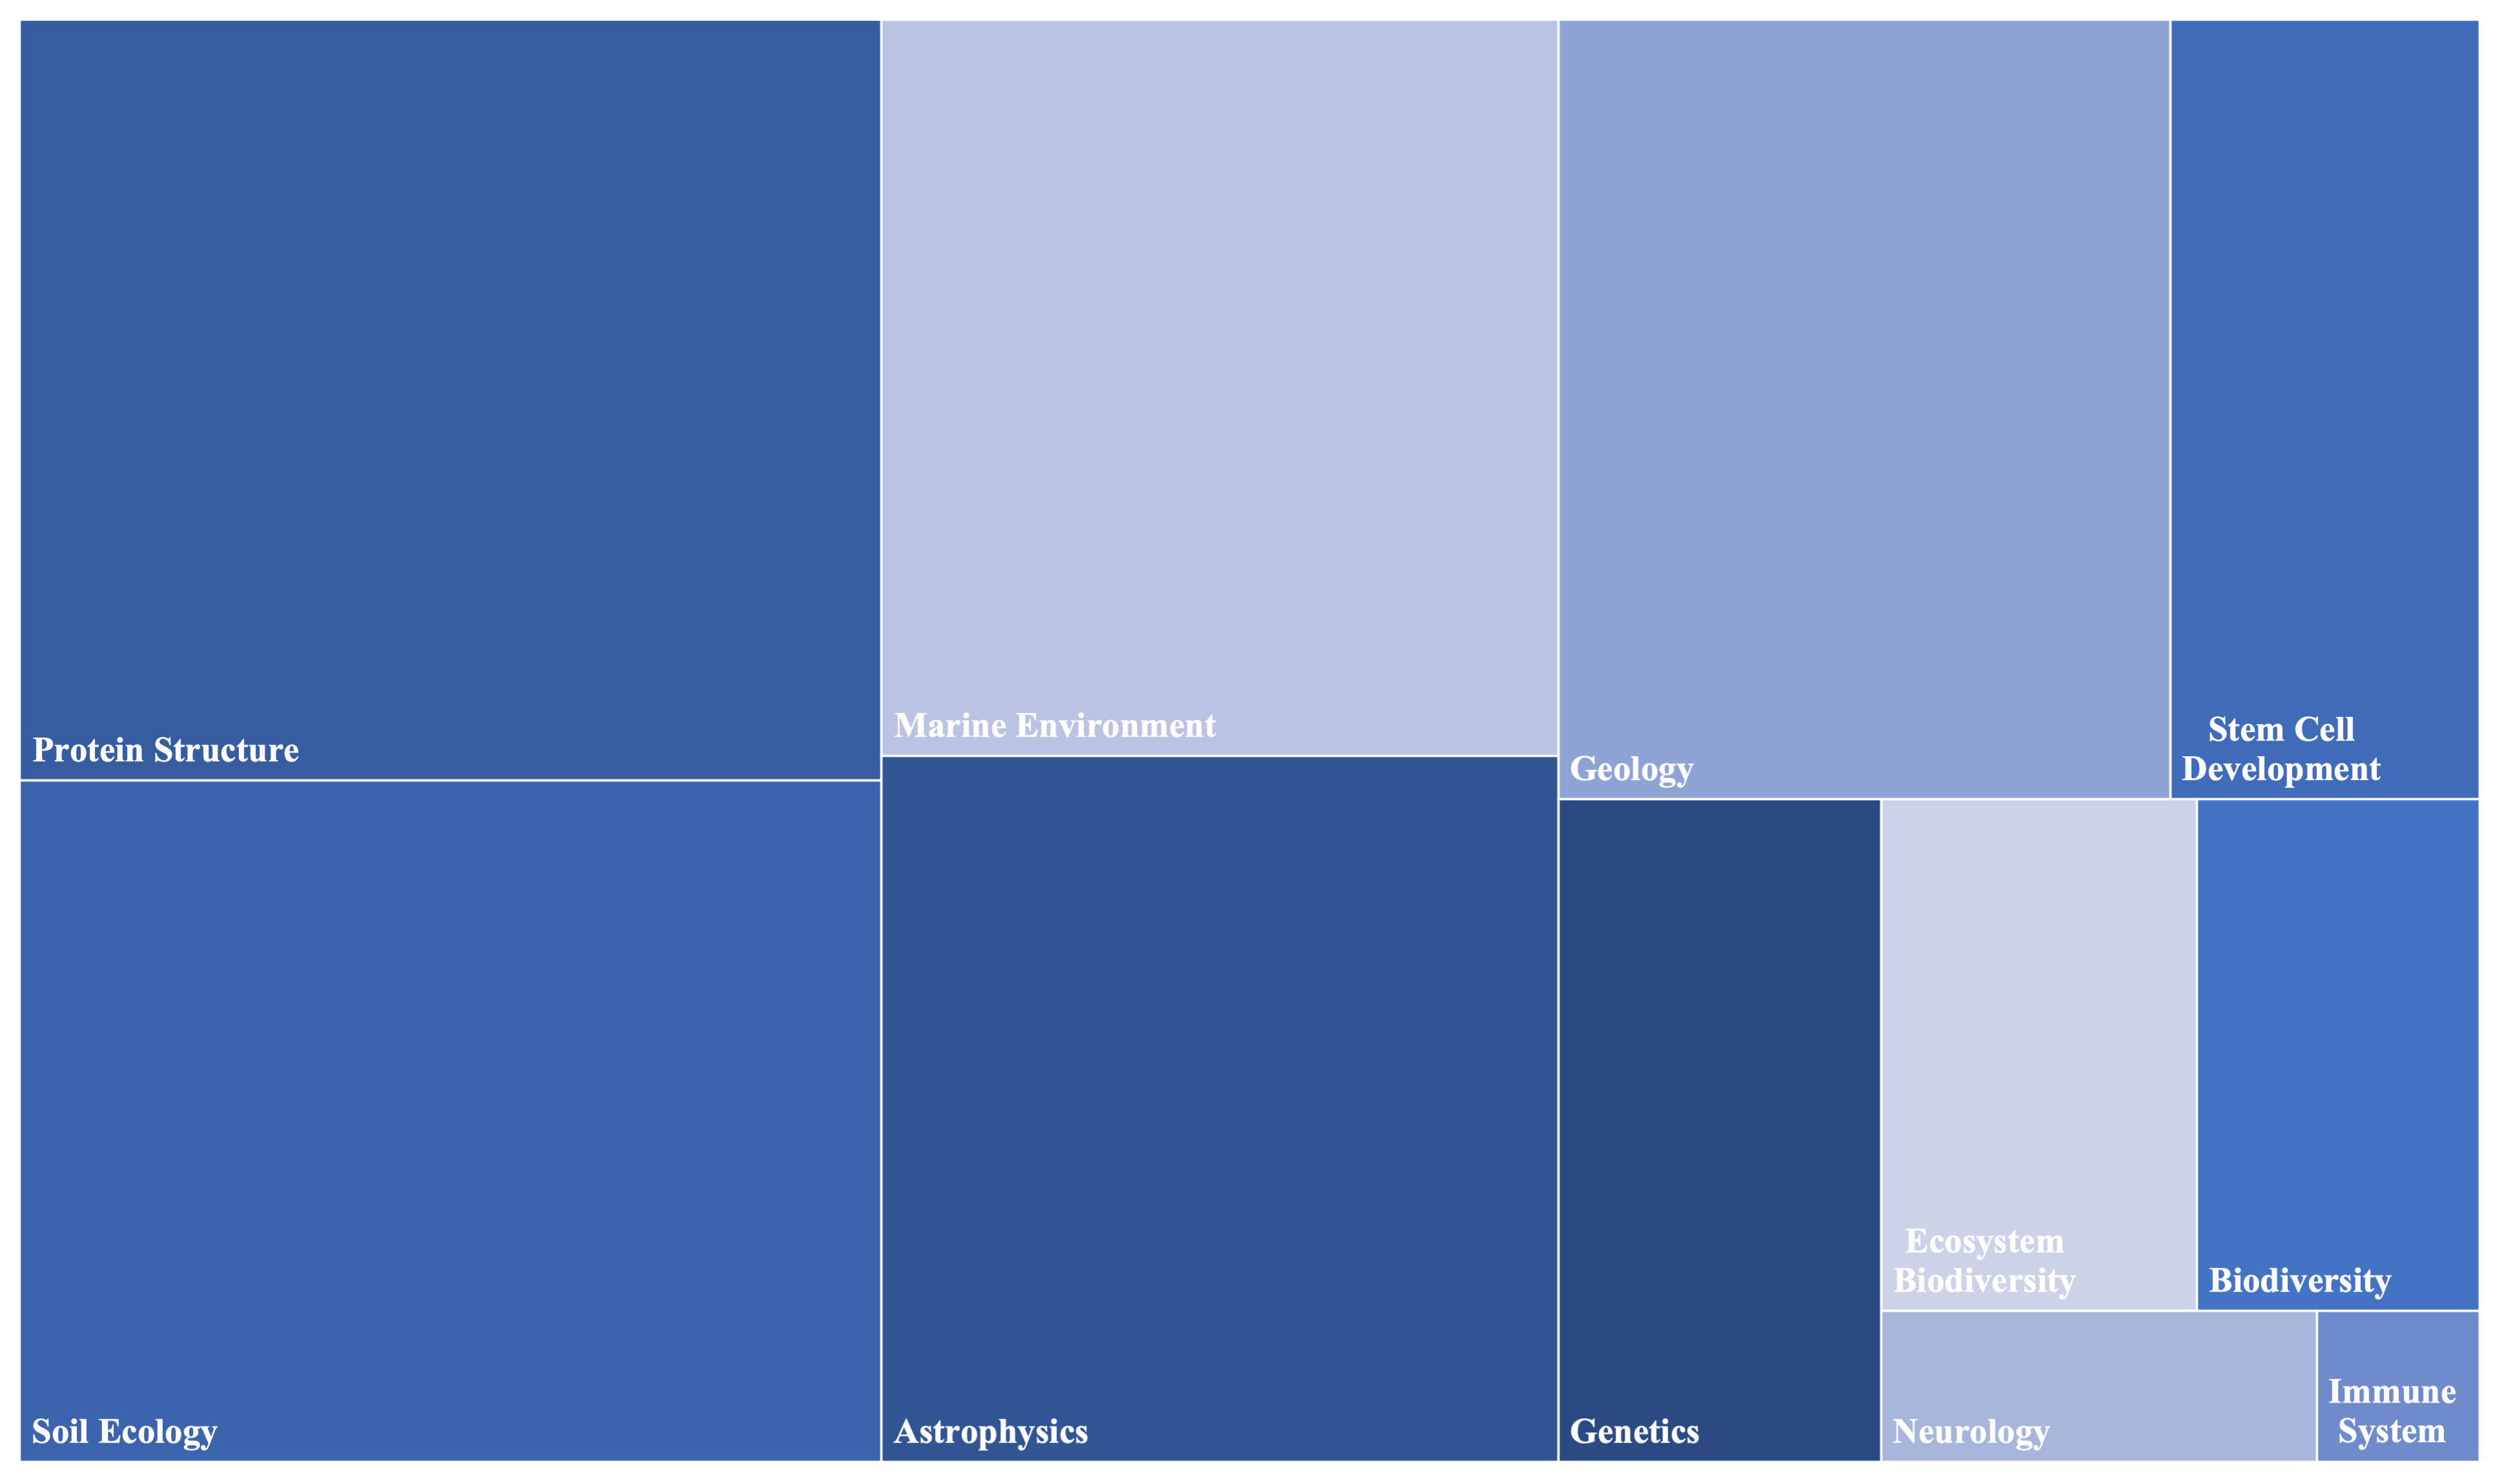
\includegraphics[width=\textwidth]{Figures/Overview of Natural Science Projects Funded in 2019-2021.png}

    \end{subfigure}
    \caption[Investment Directions within Natural Science (2013-2015 and 2016-2018)]{Within the Natural Science category, the field of Life Science consistently received a relatively higher amount of funding compared to Physical Science.}
    \label{fig3.6}
\end{figure}
%TC:endignore
Natural science can be further categorized into two main divisions: life science and physical science. Life science refers to disciplines like biology or human anatomy, essentially encompassing the scientific study of all living organisms on Earth. On the other hand, physical science encompasses the remaining natural sciences, including fields like chemistry and physics, as well as areas unrelated to life \citep{ledoux2002defining}.\\

%TC:ignore
\begin{figure}[H]
\centering
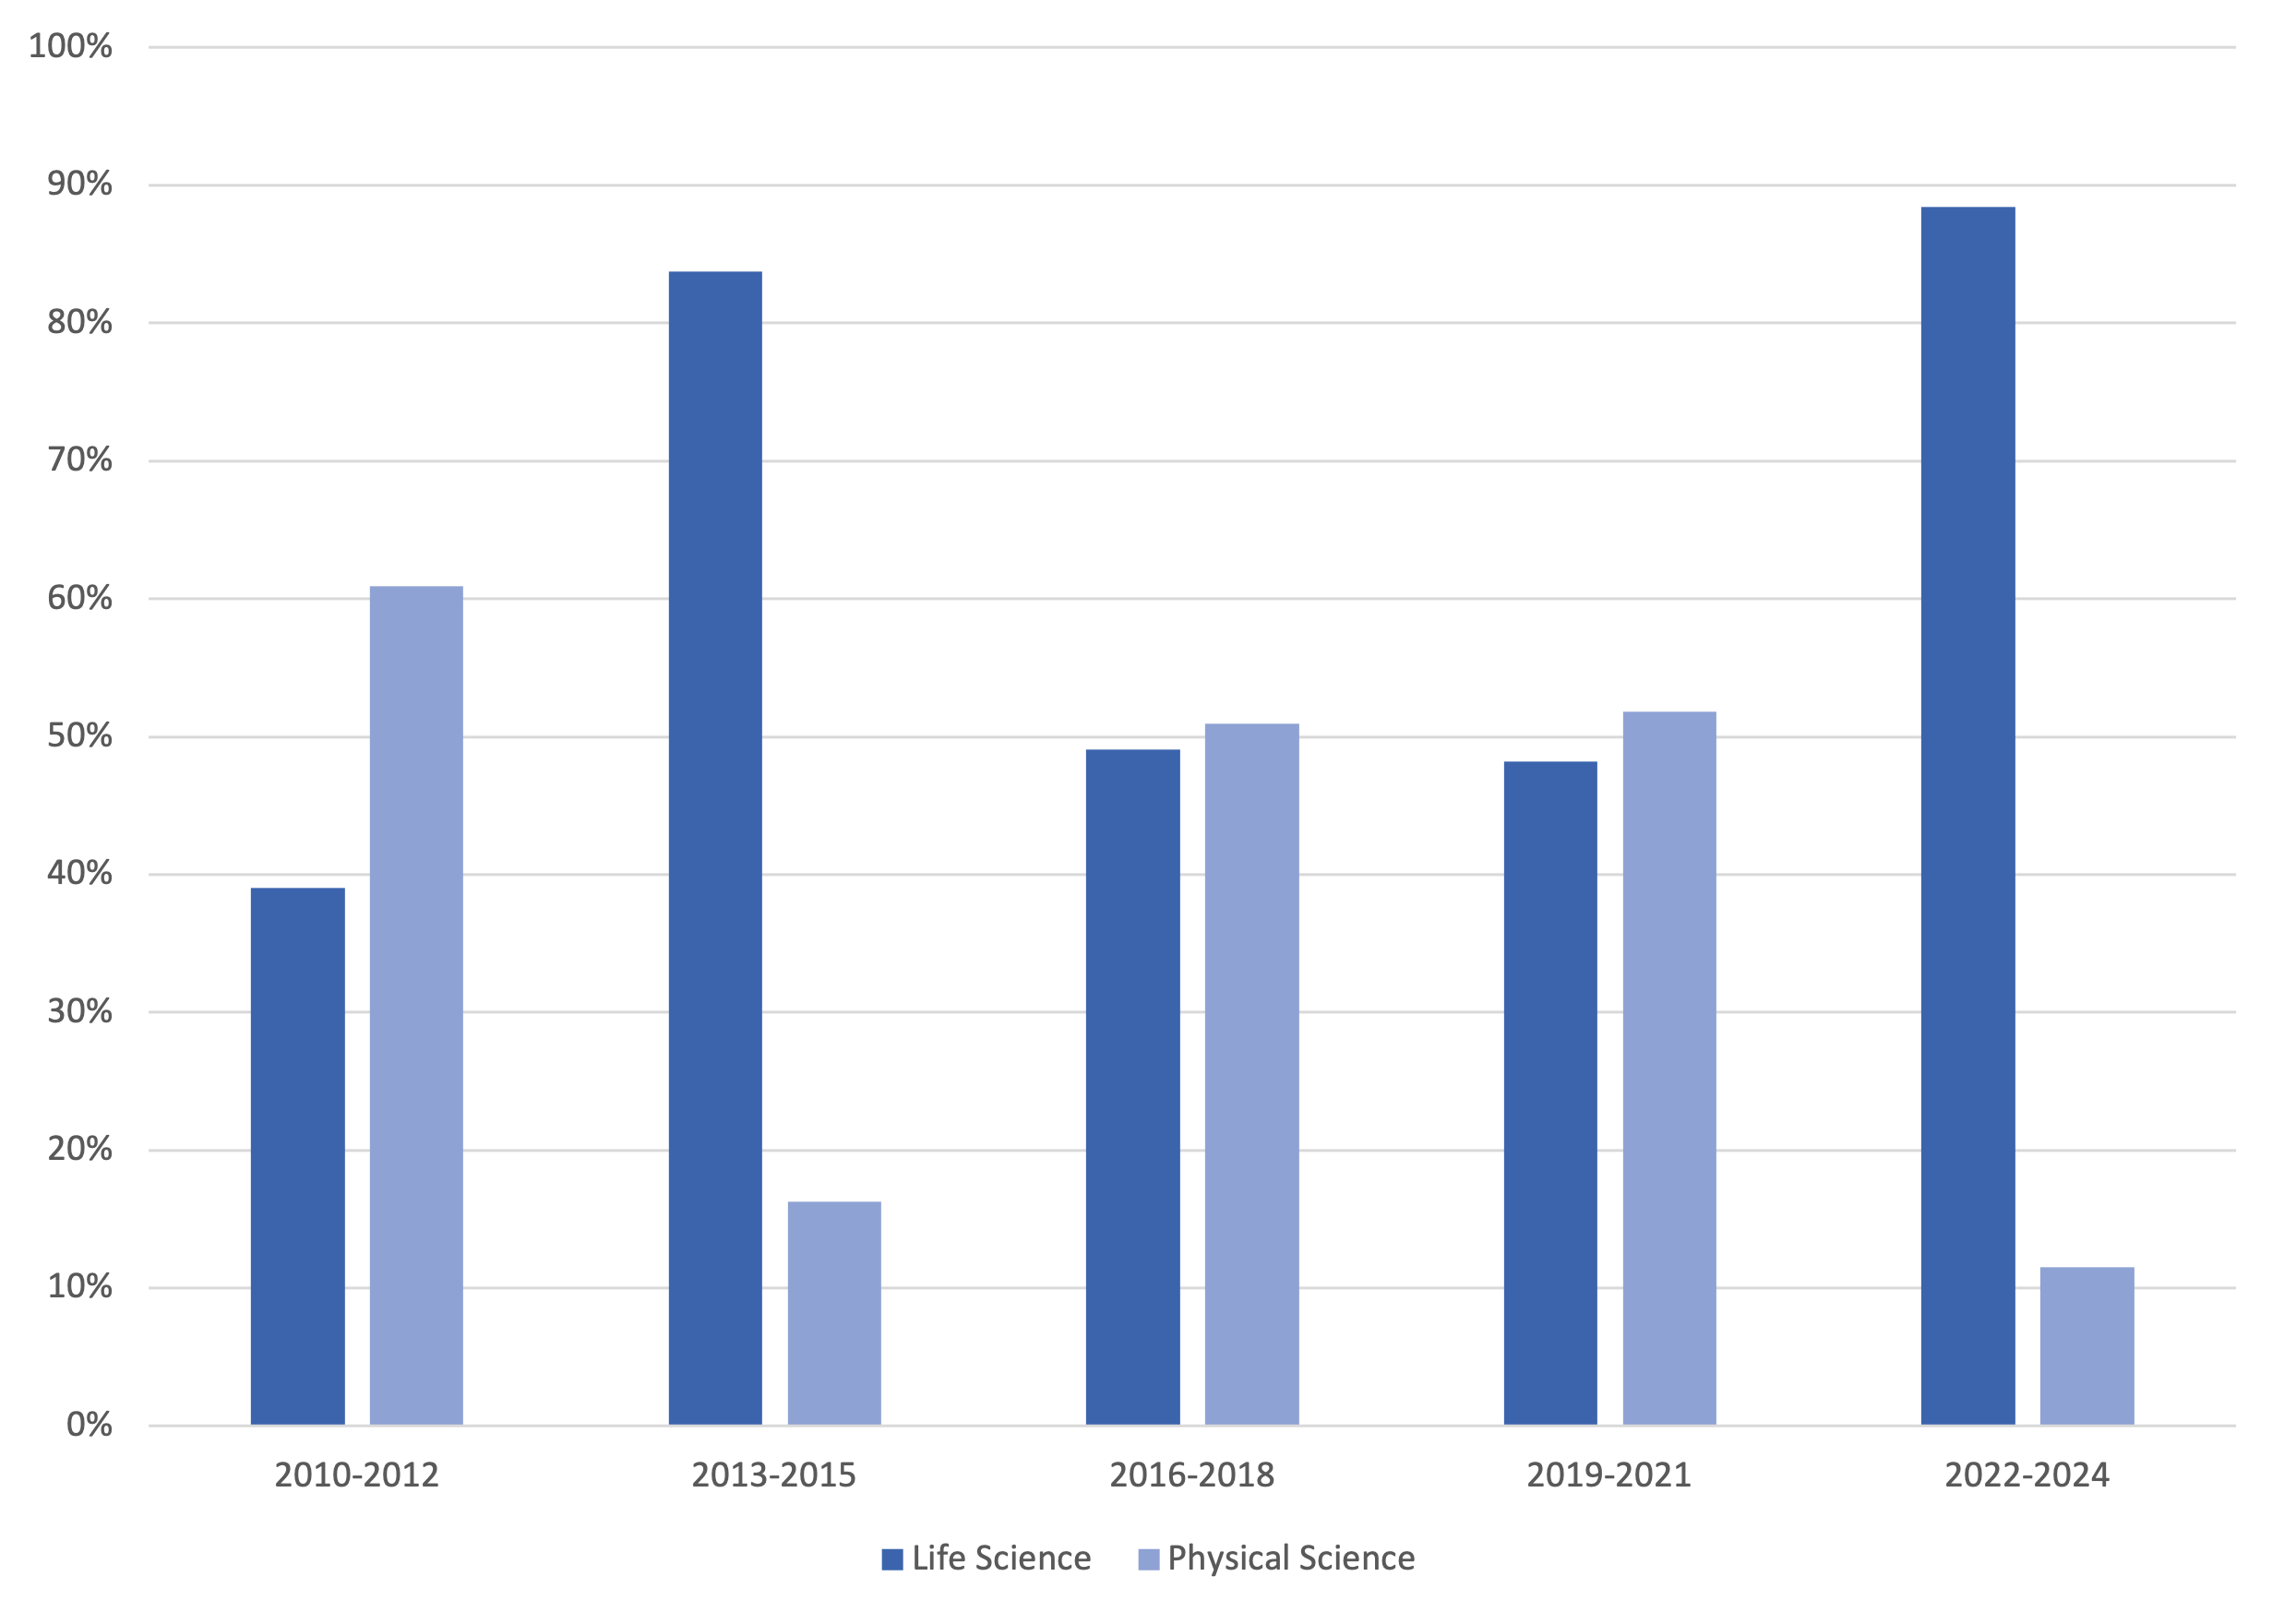
\includegraphics[scale=0.8]{ProjectReportTemplate/Figures/natural_science_prop.png}
\caption[Allocation of Funding in Natural Science]{UKRI does not show a clear preference for either life science or physical science within the category of natural science.}
\label{figure} 
\end{figure}
%TC:endignore

The data for the years 2022-2024 has provided further intriguing insights. UKRI's investment strategy during this period continues to favor natural science and applied science, reflecting a continued emphasis on these domains. Funding for specific sub-disciplines such as Public Health, Computer Science, Fluid Dynamics, and Ecology has also been sustained. However, due to the incompleteness of data for 2023 and 2024, with several projects still in the application phase, a comprehensive analysis of the funding trends for this period has not been conducted. This highlights the dynamic nature of research funding and the ongoing evolution of priorities within the funding landscape. Further investigation into these recent trends may unveil new dimensions of research support and shed light on emerging directions.\\


\section*{Evolution of Funding Amounts in Specific Disciplines}

Continuing our investigation, I delve into the intriguing landscape of disciplines that have consistently secured funding over time. While these disciplines have remained on the funding roster, the allocated amounts have fluctuated, possibly influenced by the specific financial requirements of projects during each period. By delving into these nuances, we aim to discern the intricate patterns underlying funding variations and shed light on the evolving priorities within various domains.\\

%TC:ignore
\begin{table}[H]

    \caption{Consistently Funded Research Topics Across Five Phases (2010-2024)}
    \label{tab: Topic List1}


        \begin{tabular}{ *{4}{c} } 

            \midrule
           Imaging &Genetics &Computer Science&Environmental Science \\
           Pharmaceutical Science&Particle Physics&
           Fluid Dynamics&Education\\
           Geology&Ecology&Public Health &Materials Science\\

            \bottomrule
        \end{tabular}

\end{table}
%TC:endignore

Compared to the Natural Science and Applied Science categories, which have prominently led in the number of funded projects and the allocated amounts, the domains of Social Science and Formal Science exhibit a more stable array of funded research directions. Within Formal Science, fields such as Theoretical Physics and Computer Science have consistently secured funding, reflecting their enduring significance.\\

On the other hand, Natural Science and Applied Science have encompassed a diverse spectrum of funded research domains. Notably, this diversity includes areas like Environmental Science, Ecology, Pharmaceutical Science, and various branches of Biology. Biology has emerged as a dynamic focal point, manifesting a rich tapestry of funded sub-disciplines over the past two decades. These encompass a myriad of specializations, such as Cell Biology, Molecular Biology, Microbiology, and more.\\

Furthermore, "Public Policy" stands as a distinctive current within the realm of Social Science, representing a significant recipient of funding. Notably, within the broader landscape of Social Science, "Public Policy" consistently demonstrates a relatively higher probability of securing funding. This prominence underscores this field's vital role in shaping and informing societal decisions, governance, and strategies.\\

Indeed, the disparity in funding amounts across various domains does not inherently reflect the differing levels of emphasis by UKRI. The allocation of funds is largely influenced by the financial requirements of individual projects. Certain research fields necessitate substantial financial investments due to the costs associated with experimental equipment, while other domains, such as purely theoretical research, might have relatively lower demands for resources.\\


%TC:ignore
\begin{figure}[H]
    \centering
    \begin{subfigure}{\textwidth}
        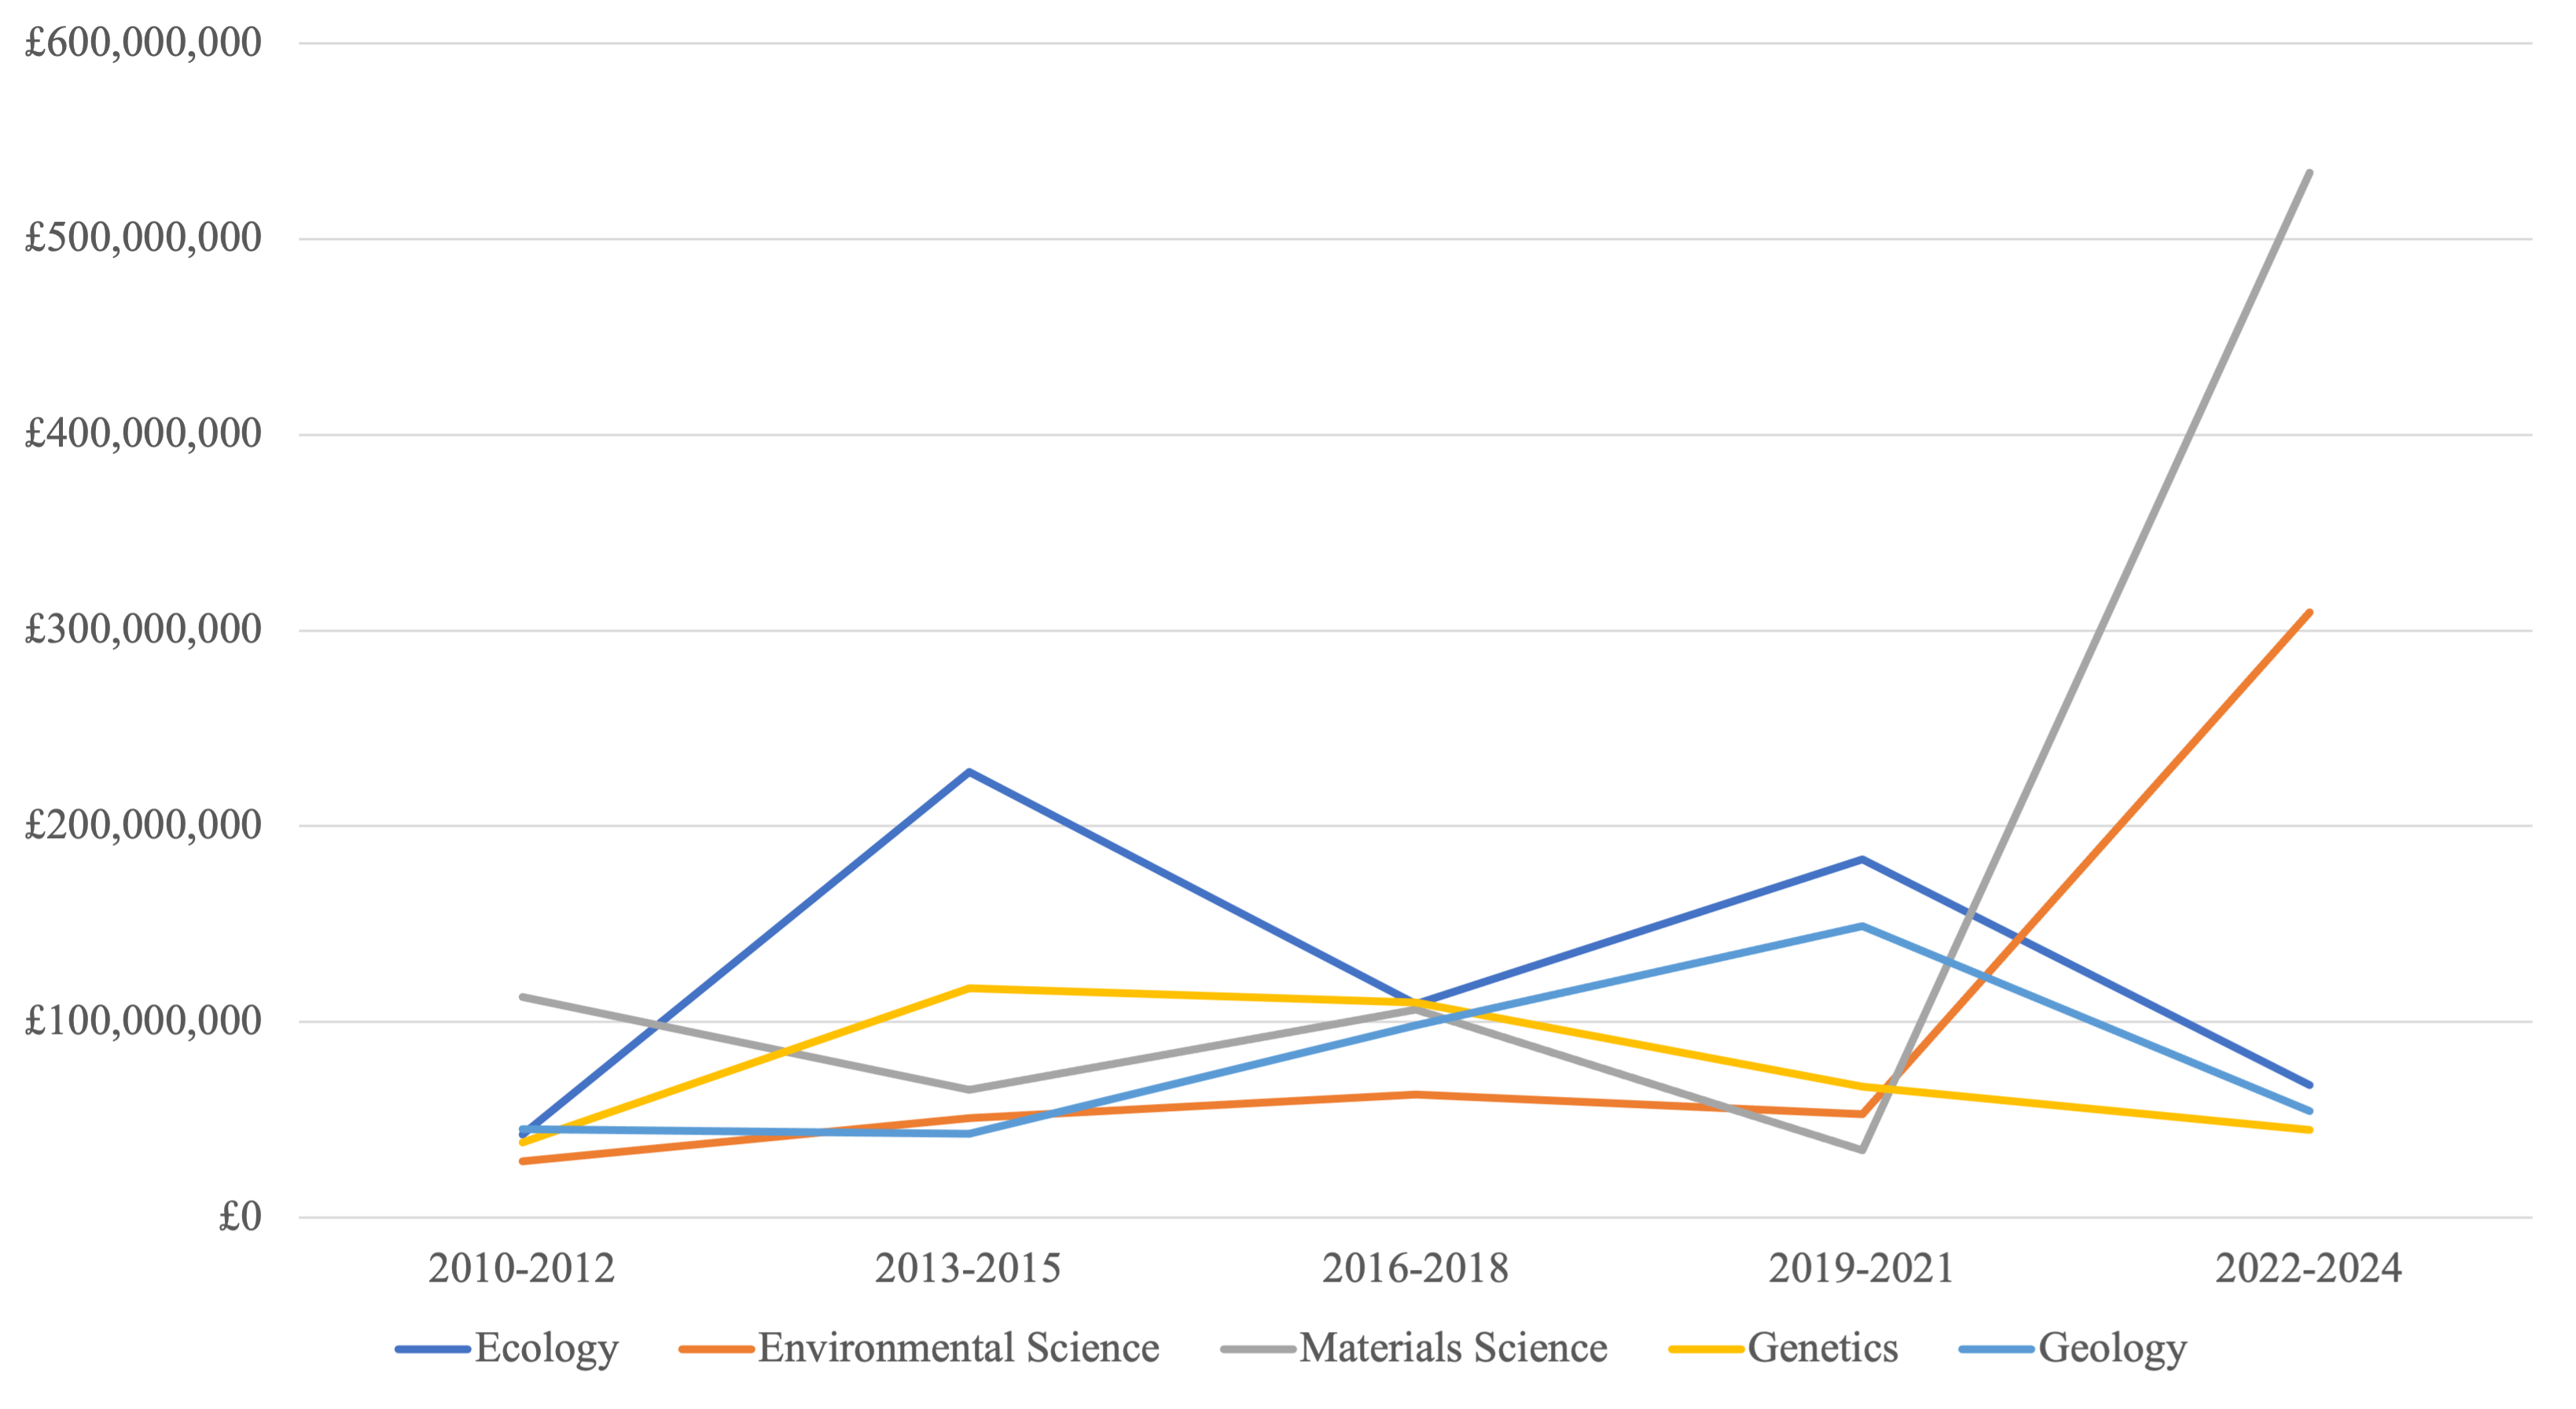
\includegraphics[width=0.8\textwidth]{Figures/Natural Science Funding Trends.png}
       
        \label{fig:2016-2018}
    \end{subfigure}

    \begin{subfigure}{\textwidth}
        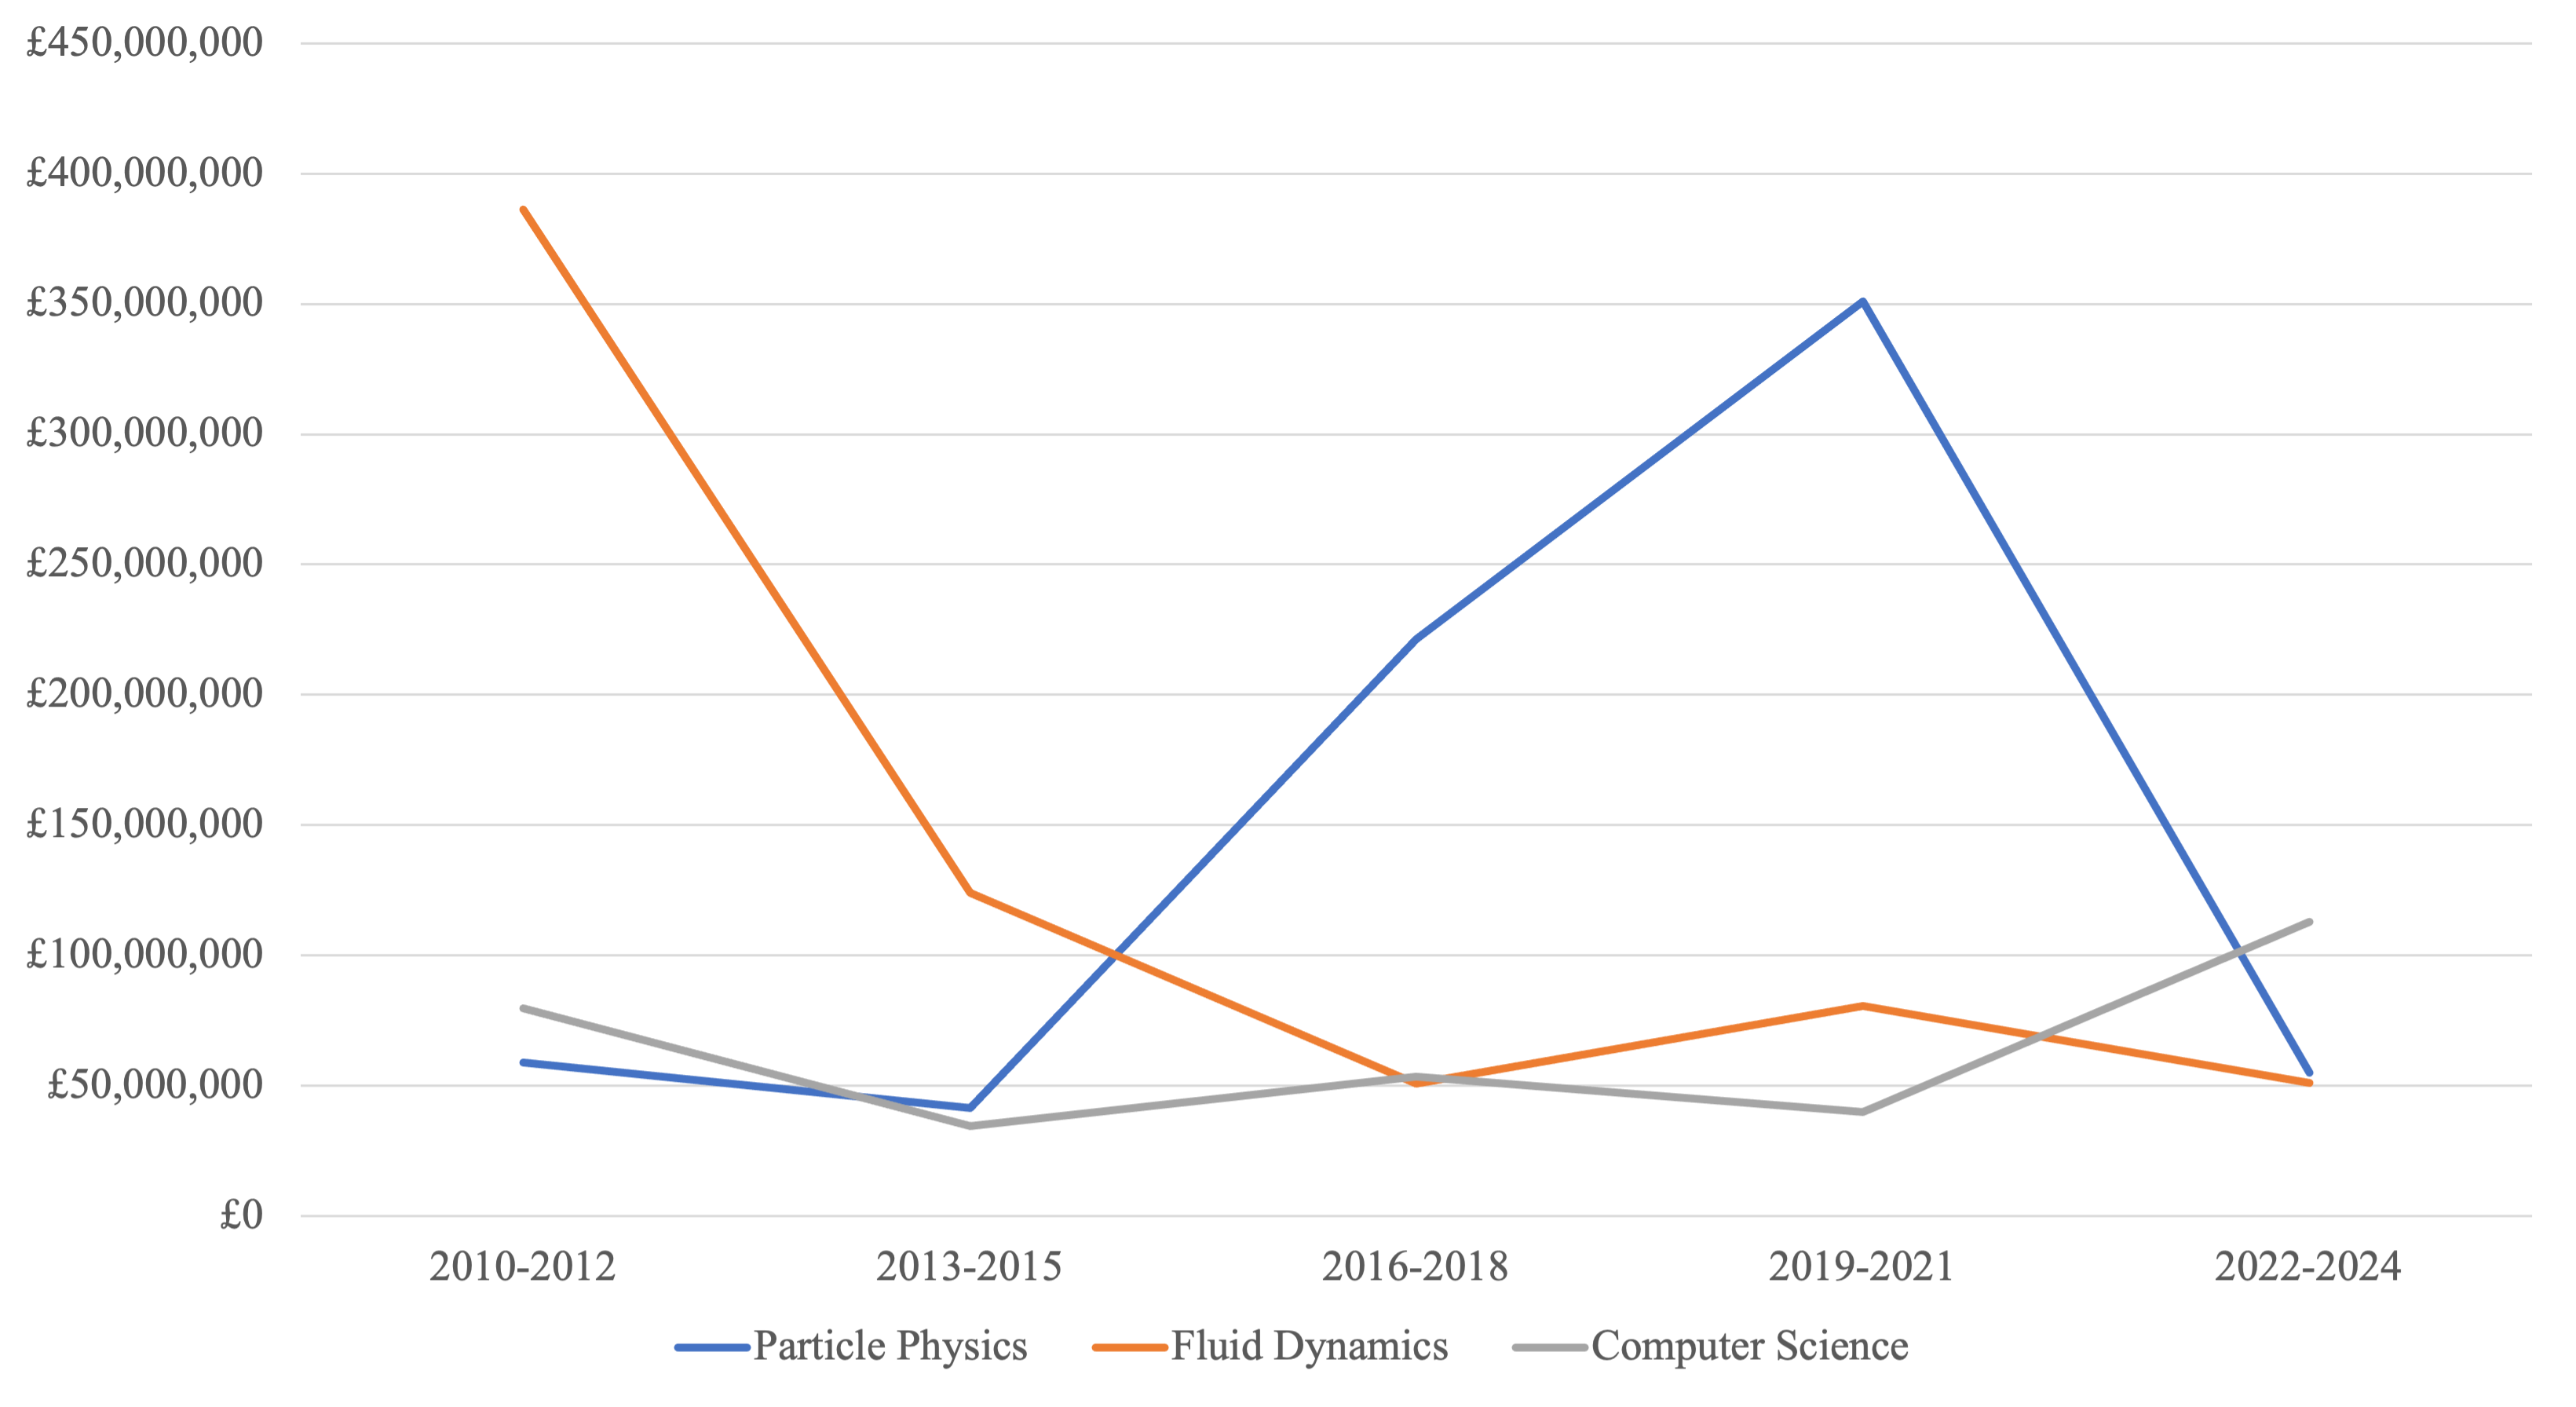
\includegraphics[width=0.8\textwidth]{Figures/Formal Science Funding Trends.png}
       
        \label{fig:2019-2021}
    \end{subfigure}
    \caption[While these directions have received consistent financial support, none of them exhibit a clear growth trend.]{Changing Fortunes in Science Funding}
    \label{fig3.8}
\end{figure}
%TC:endignore

Despite continuous funding support from UKRI over 21 years, there is no discernible consistent pattern in funding amounts for these research directions. Each direction has experienced significant fluctuations in funding levels. Notably, most projects within natural science have consistently received funding around or below 200,000,000. This suggests that while natural science projects contribute to the overall funding pool, the allocation per individual direction remains relatively modest. Within this context, it is worth highlighting that ecology has consistently outperformed other directions in terms of funding amounts, indicating promising prospects for the field.\\

